\capitulo{5}{Aspectos relevantes del desarrollo del proyecto}

En esta sección, se destacarán los elementos más significativos del desarrollo, proporcionando una perspectiva detallada de las decisiones adoptadas para alcanzar los objetivos del proyecto. Se resumirá la experiencia práctica, detallando cómo se abordaron los desafíos específicos, y se evaluará la importancia de estas soluciones en el contexto general del alcance del proyecto.

\section{Motivación del proyecto}

La motivación subyacente a este proyecto surge de la creciente importancia y demanda en el ámbito de la monitorización de invernaderos, especialmente en el contexto del cultivo de cannabis medicinal. La necesidad de implementar soluciones tecnológicas eficientes para garantizar condiciones óptimas de cultivo y maximizar la producción ha impulsado la elección de este tema.

El objetivo principal radica en diseñar un sistema económico y eficaz que permita a los cultivadores de cannabis medicinal supervisar las condiciones ambientales de sus invernaderos de manera remota. Este proyecto busca proporcionar una herramienta valiosa para mejorar la eficiencia, la calidad y la consistencia en la producción de cannabis medicinal, al tiempo que se abordan los desafíos específicos asociados con la monitorización de variables críticas como temperatura, humedad y luz.

\section{Formación necesaria}

El proyecto ha requerido una formación interdisciplinaria que abarca diversas áreas. En primer lugar, la comprensión profunda de los principios de la programación y el desarrollo de software ha sido esencial. La elección de la Raspberry Pi Pico W como plataforma y la programación en MicroPython para controlar los dispositivos hardware involucra un conocimiento sólido en programación embebida y desarrollo en entornos limitados.

Además, la utilización de sensores especializados, como el DHT22~\cite{manual:DHT22}, el BH1750~\cite{manual:BH1750} y el sensor de humedad del suelo~\cite{wiki:SensorHumedadSuelo}, ha demandado una comprensión detallada de los principios de operación de estos dispositivos y cómo integrar sus lecturas en el sistema general. Esto implica una formación técnica en electrónica y sensores.

La implementación de conceptos relacionados con el Internet de las cosas (IoT) y la comunicación inalámbrica mediante la Raspberry Pi Pico W~\cite{misc:RPiPicoW} también ha requerido conocimientos específicos en redes y protocolos de comunicación.

La integración de MQTT~\cite{manual:MQTT} en el código MicroPython para la Raspberry Pi Pico W ha requerido conocimientos específicos sobre este protocolo de mensajería ligero diseñado para la eficiente comunicación entre dispositivos en redes IoT.

En resumen, la formación necesaria abarca habilidades en programación embebida, electrónica, redes, IoT y desarrollo de software. La combinación de estas competencias ha sido esencial para la ejecución exitosa del proyecto, demostrando la importancia de una formación integral y multidisciplinaria en el ámbito de la ingeniería y la tecnología.
\pagebreak

\section{Metodología}
Se ha optado por la metodología del \textbf{Modelo de Prototipos}~\cite{misc:Metodologia_ModeloDePrototipos} debido a su capacidad para proporcionar retroalimentación temprana, clarificar requisitos, adaptarse a cambios, validar prácticamente funcionalidades, reducir riesgos, comprender la interfaz de usuario y facilitar la mejora continua. Este enfoque iterativo permite identificar y corregir problemas desde las primeras etapas, garantizando la eficiencia y el éxito en el desarrollo del sistema IoT de monitorización de invernaderos de cannabis medicinal.

\subsection{Identificación de Requisitos Iniciales:}
\textbf{Hardware:}
\begin{itemize}
	\item Raspberry Pi Pico W~\cite{misc:RPiPicoW} como la plataforma central.
	\item Sensores DHT22~\cite{manual:DHT22} para medir temperatura y humedad ambiente.
	\item Sensor BH1750~\cite{manual:BH1750} para evaluar la intensidad de luz.
	\item Sensor de humedad de suelo~\cite{wiki:SensorHumedadSuelo} para monitorizar las condiciones del suelo.
	\item Pantalla OLED~\cite{manual:Oled} para visualización de datos.
	\item LEDs RGB~\cite{manual:LedRGB} para indicar condiciones críticas.
\end{itemize}

\textbf{Software:}
\begin{itemize}
	\item Desarrollo de un sistema en MicroPython para la Raspberry Pi Pico W~\ref{proyecto:Hardware}.
	\item Implementación de un servidor LAMP para almacenar y gestionar datos.
	\item Integración de la API de Telegram~\cite{misc:Telegram_api} para recibir alertas.
	\item Aplicación de escritorio para Windows~\ref{proyecto:InverIoT}, desarrollada en Visual Studio 2022 en lenguaje C\#. Incluye su instalador.
	\item Dashboard web~\ref{proyecto:Dashboard}, realizado con Node.js, accesible desde internet.
\end{itemize}

\textbf{Funcionalidades clave:}
\begin{itemize}
	\item Captura de datos ambientales como temperatura, humedad, luz y humedad del suelo.
	\item Representación gráfica de los datos en una pantalla OLED.
	\item Envío de alertas a través de Telegram en caso de valores fuera de los umbrales ideales.
	\item Interacción bidireccional para activar mecanismos de respuesta a condiciones ambientales adversas.
\end{itemize}

\subsection{Desarrollo del Primer Prototipo:}
En esta etapa, se enfocó en la integración de los componentes hardware definidos, como la Raspberry Pi Pico W~\cite{misc:RPiPicoW} y los sensores de humedad, temperatura~\cite{manual:DHT22}, luminosidad~\cite{manual:BH1750} y humedad del suelo~\cite{wiki:SensorHumedadSuelo}. Se estableció la conexión con el servidor LAMP utilizando MQTT~\cite{manual:MQTT} para la transmisión de datos en tiempo real.

Durante la fase de desarrollo, se configuraron y probaron los mecanismos de alerta a través del bot de Telegram y la activación de los LEDs RGB para indicar condiciones críticas. También se diseñó e implementó la lógica de umbrales para verificar si los valores ambientales están dentro de los límites ideales.

\subsection{Evaluación del Primer Prototipo:}
El objetivo principal fue validar la efectividad de las funcionalidades implementadas y su capacidad para cumplir con los requisitos planteados en la fase inicial del proyecto.
\begin{itemize}
	\item \textbf{Pruebas de Mecanismos de Alerta y Retroalimentación Visual:}
Se realizaron pruebas del sistema de alertas a través del bot de Telegram. Se verificó la capacidad del sistema para enviar notificaciones en tiempo real sobre condiciones ambientales críticas, como temperaturas extremas o niveles de humedad fuera de los umbrales establecidos.

Además, se evaluó la respuesta de los LEDs RGB conectados, los cuales indican visualmente las condiciones del entorno. Cada color del LED se asoció con un estado específico, permitiendo una retroalimentación instantánea sobre el estado actual del invernadero.
\item \textbf{Verificación de la Lógica de Umbrales:}
La lógica de umbrales, diseñada para verificar si los valores ambientales se mantienen dentro de los límites ideales, está en fase de pruebas en un entorno no controlado. En este contexto, se observa que los valores experimentan salidas fuera de los umbrales establecidos. Sin embargo, se ha verificado con éxito que la lógica implementada para activar las alertas funciona de manera efectiva cuando los valores se desvían de los límites ideales predefinidos.
\end{itemize}
\subsection{Retroalimentación y Mejoras:}
Tras la evaluación del primer prototipo, se recopiló retroalimentación valiosa para orientar mejoras futuras. Se identificaron áreas de oportunidad, como la necesidad de ajustar los umbrales para adaptarse a condiciones específicas del entorno y mejorar la precisión de las alertas. La retroalimentación del usuario sobre la interfaz y la usabilidad también se tuvo en cuenta para realizar ajustes en el diseño del dashboard web y la aplicación de escritorio. Estas observaciones se utilizarán como guía para la siguiente iteración del prototipo, buscando una mayor eficiencia y adecuación a los requisitos específicos del sistema.

\subsection{Desarrollo de Subsiguientes Prototipos:}
Con base en la retroalimentación obtenida del primer prototipo, se inició el desarrollo de subsiguientes prototipos con el objetivo de implementar mejoras significativas. Se priorizó la optimización de los umbrales de alerta, considerando las condiciones específicas del entorno de monitoreo. También se abordaron ajustes en la interfaz del dashboard web y la aplicación de escritorio, respondiendo a las sugerencias de los usuarios para mejorar la usabilidad y la experiencia general. Cada nuevo prototipo se sometió a pruebas exhaustivas para validar las mejoras implementadas y garantizar un funcionamiento más eficiente del sistema en su conjunto. Este proceso iterativo permitió refinamientos continuos, enfocados en lograr un sistema de monitoreo más preciso y adaptado a las necesidades específicas del usuario.

\subsection{Validación Continua:}
Se llevaron a cabo pruebas exhaustivas para verificar el funcionamiento del sistema, evaluando diversos escenarios y condiciones ambientales para confirmar la precisión de los sensores y la respuesta del sistema. Se realizaron pruebas de estrés para evaluar la capacidad de respuesta en situaciones extremas.

Durante un período prolongado, se recopilaron datos para analizar el rendimiento a lo largo del tiempo, comparándolos con los umbrales ideales establecidos. Algunos valores se salieron del rango ideal debido a las pruebas en un entorno no controlado, pero se verificó que el sistema funcionó correctamente y generó alertas de manera adecuada al encontrarse en un ambiente controlado.

La retroalimentación continua de las pruebas y la validación de los resultados se utilizaron para ajustar el sistema, mejorando su robustez y confiabilidad. Este ciclo de validación y ajuste continuo contribuyó a optimizar el sistema para lograr un monitoreo preciso y eficiente de las condiciones del invernadero.

\subsection{Integración de Componentes:}
Durante esta etapa, se procedió a la integración de los diferentes componentes del sistema. Se conectaron y configuraron la Raspberry Pi Pico W~\cite{misc:RPiPicoW} como plataforma central, junto con los sensores DHT22, BH1750~\cite{manual:BH1750} y el sensor de humedad del suelo~\cite{wiki:SensorHumedadSuelo}. Se aseguró la comunicación efectiva entre estos elementos, permitiendo la captura precisa de datos ambientales.

El desarrollo de un sistema en MicroPython~\cite{wiki:micropython} para la Raspberry Pi Pico W se integró con éxito con el servidor LAMP, facilitando la gestión y almacenamiento de datos. La implementación de la API de Telegram~\cite{misc:Telegram_api} se conectó con el sistema para recibir alertas en tiempo real.

La aplicación de escritorio para Windows~\ref{proyecto:InverIoT}, desarrollada en Visual Studio 2022 con lenguaje C\#~\cite{manual:CSharp}, se integró sin problemas, permitiendo la visualización de datos en tiempo real y la interacción bidireccional con el sistema.

El dashboard web~\ref{proyecto:Dashboard}, creado con Node.js, se integró para ofrecer una interfaz accesible a través de internet, proporcionando una visualización completa y en tiempo real de los datos capturados. Esta etapa de integración aseguró la cohesión y el funcionamiento conjunto de todos los componentes del sistema IoT para el monitoreo de invernaderos.

\subsection{Ajustes Finales:}
Estos ajustes se centraron en mejorar la precisión de los sensores, la eficacia de las alertas y la respuesta de los mecanismos de control. Se llevaron a cabo modificaciones en el código del sistema para perfeccionar la lógica de umbrales y asegurar que los valores se mantuvieran dentro de los límites ideales.

Además, se realizaron ajustes en la configuración de la pantalla OLED y los LEDs RGB para una visualización más clara y distintiva de las condiciones del invernadero. La interfaz de usuario se mejoró para facilitar la comprensión de los datos mostrados en tiempo real. También se realizaron pruebas adicionales para verificar la estabilidad del sistema en condiciones diversas.

Este proceso de ajustes finales contribuyó a la optimización global del sistema, asegurando un monitoreo preciso y una respuesta efectiva a las variaciones ambientales en el invernadero. La retroalimentación continua y la iteración fueron fundamentales en esta fase para lograr un prototipo final robusto y funcional.

\subsection{Documentación:}
Se elaboró una documentación completa que abarca aspectos técnicos, funcionales y de implementación del sistema desarrollado. La documentación detallada incluye manuales de usuario para las distintas interfaces, descripciones técnicas de hardware y software, así como instrucciones para la instalación y configuración del sistema.

Además, se generaron documentos específicos para el mantenimiento del sistema, facilitando futuras actualizaciones y mejoras.

Esta documentación sirve como recurso integral para cualquier persona que interactúe con el sistema, desde usuarios finales hasta desarrolladores o técnicos de mantenimiento. Su elaboración garantiza la comprensión y el uso efectivo del sistema, contribuyendo a su sostenibilidad a lo largo del tiempo.

\subsection{Implementación Final:}
La implementación final del sistema se llevó a cabo tras la validación y ajustes continuos a lo largo de las fases de desarrollo y prototipado. En esta etapa, se consolidaron todas las funcionalidades y características planificadas, integrando los componentes hardware y software de manera coherente.

Se realizó una verificación exhaustiva de la interacción entre los sensores, la Raspberry Pi Pico W, la pantalla OLED, y los LEDs RGB. Se mejoró la respuesta del sistema ante condiciones ambientales diversas y se afinaron los algoritmos de control para garantizar un monitoreo preciso y eficiente del invernadero.

Además, se implementaron las últimas medidas de seguridad y se realizaron pruebas exhaustivas para garantizar la estabilidad del sistema en distintos escenarios. Se documentaron detalladamente los pasos necesarios para replicar la implementación final, asegurando una fácil reproducción y mantenimiento.

La implementación final refleja la evolución del sistema desde su concepción hasta la etapa de producción, consolidando todas las lecciones aprendidas durante el desarrollo y prototipado.

\section{Desarrollo del proyecto}

El propósito inicial radicaba en la recopilación de datos ambientales, tales como humedad, temperatura, intensidad de luz y humedad del suelo, con el fin de almacenarlos y presentarlos de manera gráfica.

Con este propósito, se optó por la Raspberry Pi Pico W debido a su eficiencia energética y coste accesible. Se conectaron al sistema un sensor de humedad y temperatura DHT22~\cite{manual:DHT22}, un sensor de intensidad de luz BH1750~\cite{manual:BH1750}, y un sensor de humedad de suelo~\cite{wiki:SensorHumedadSuelo}. Además, se incorporaron LEDs RGB~\cite{manual:LedRGB} para señalizar alertas. A esta parte del proyecto se ha llamado \textbf{Hardware}~\ref{proyecto:Hardware}.

\begin{figure}[h]
	\centering
	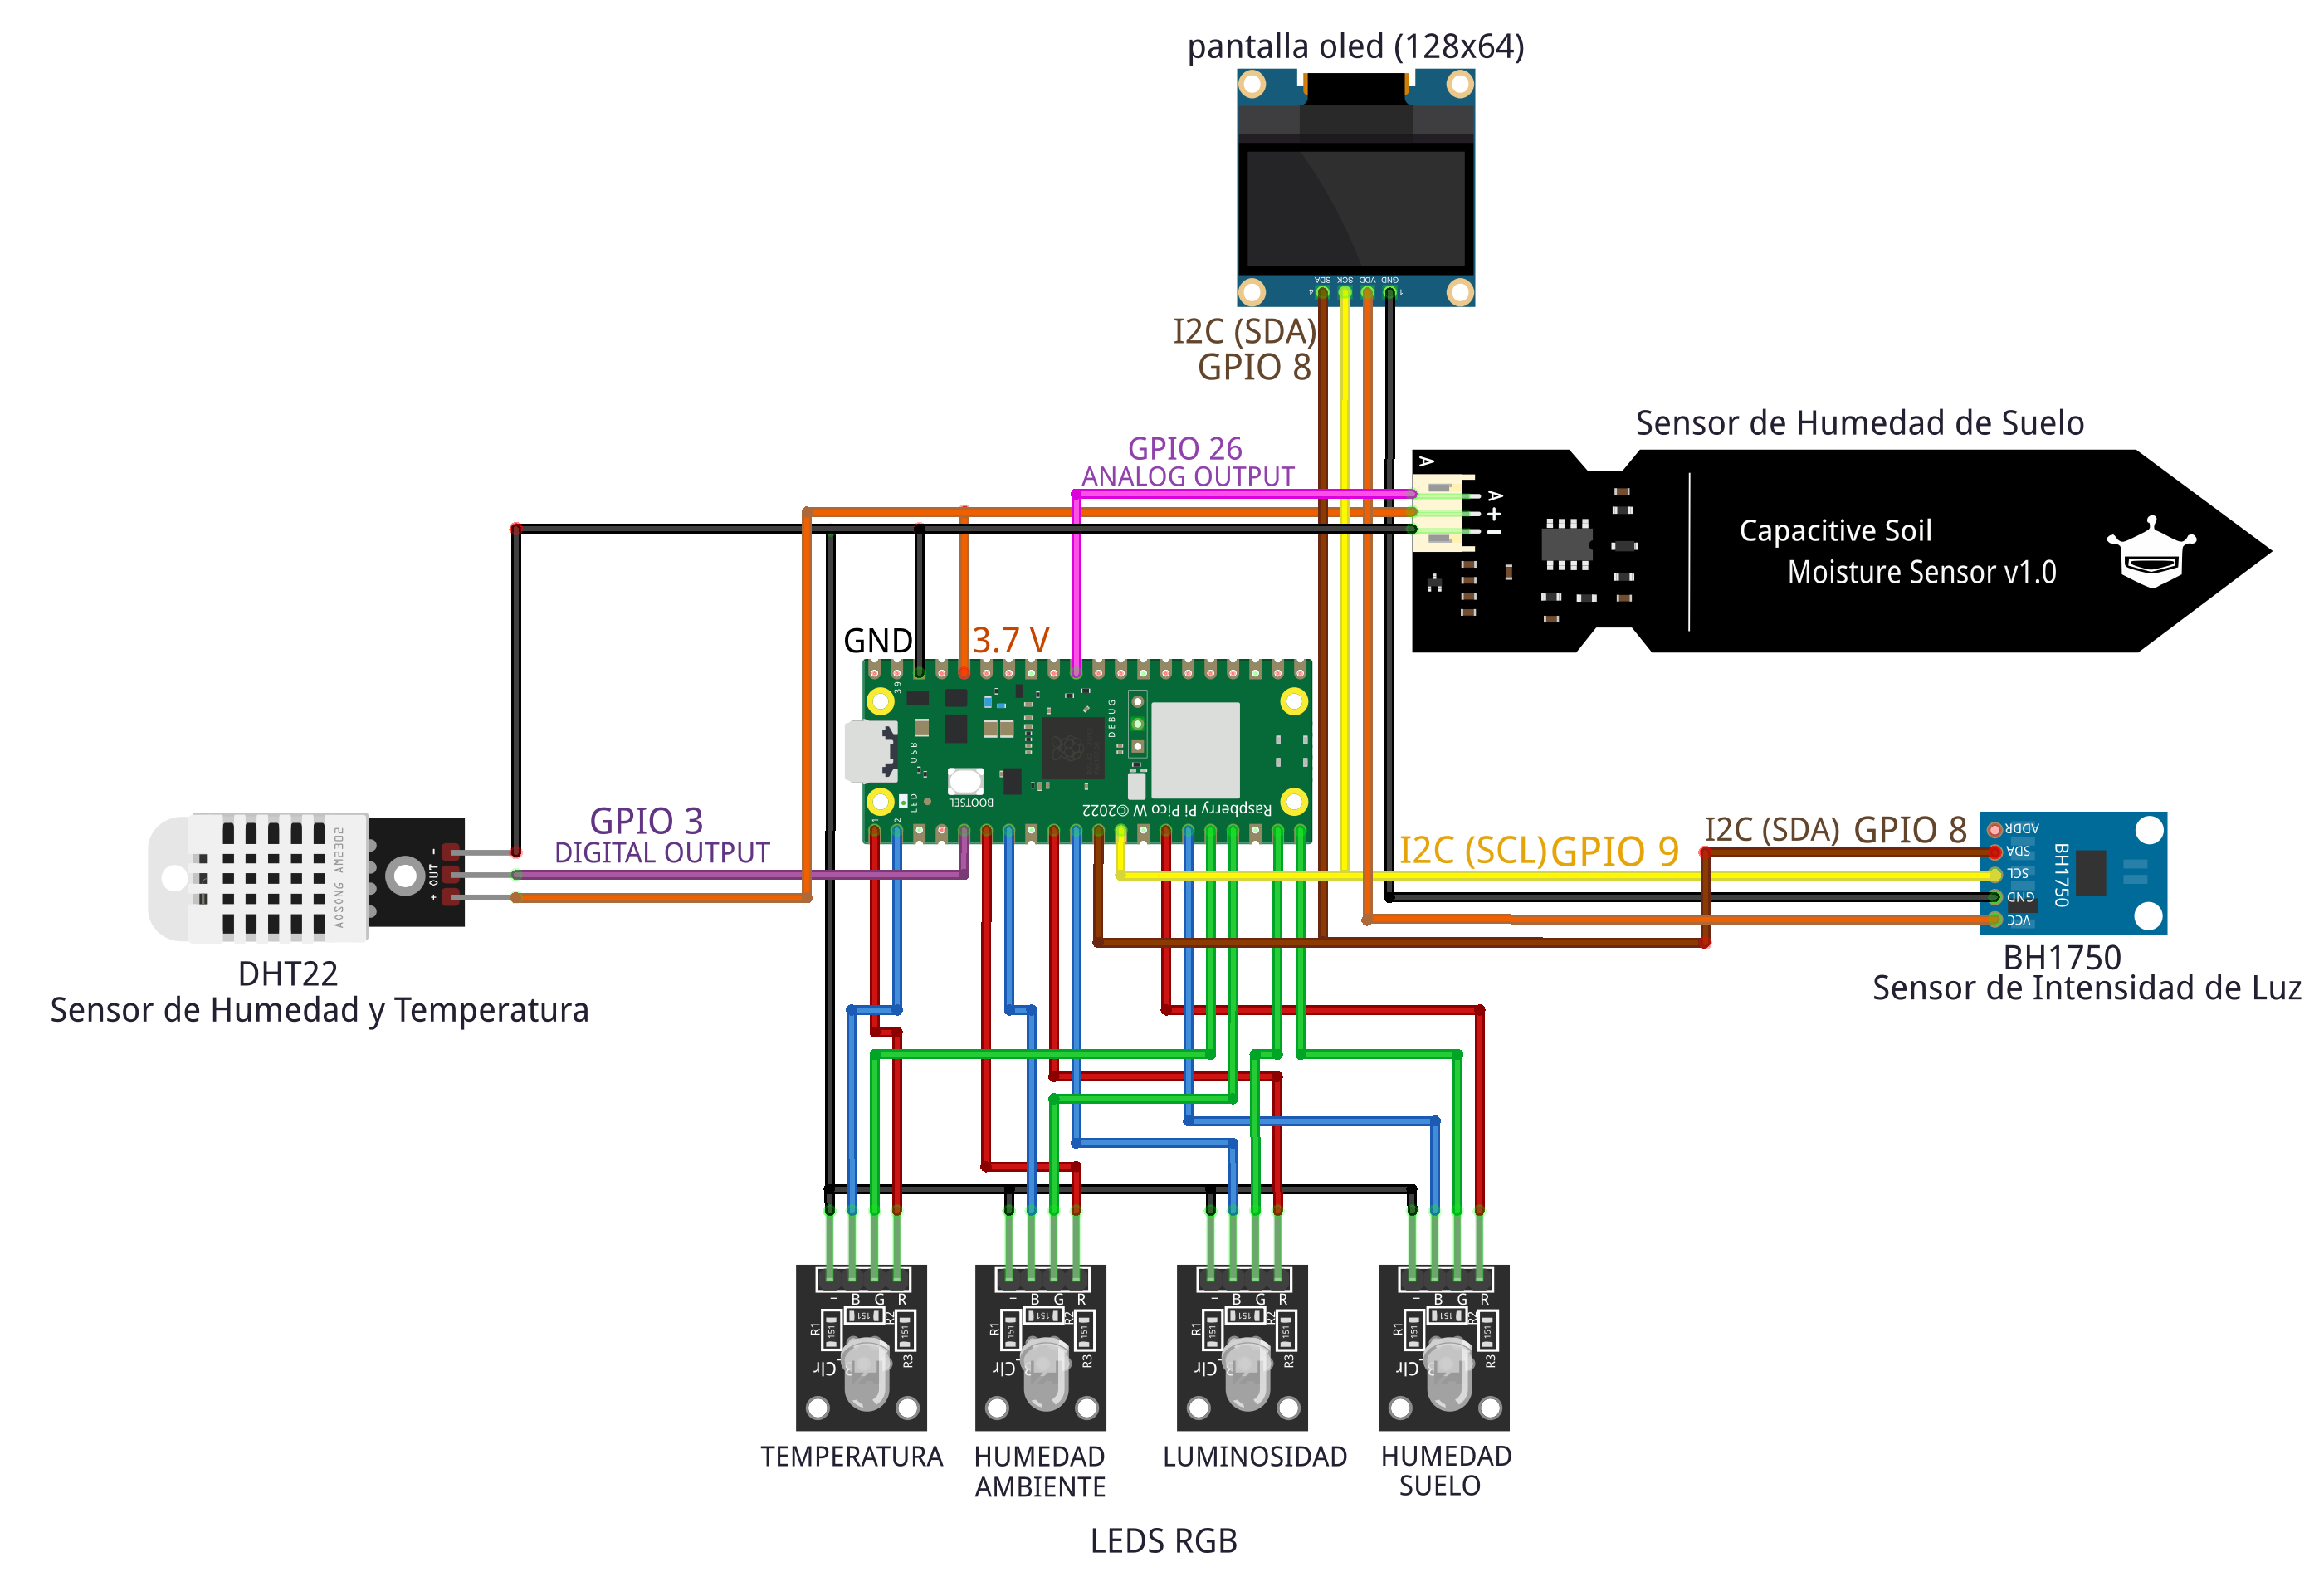
\includegraphics[width=0.8\textwidth]{img/diagramas/conexiones_simple.png}
	\caption{Raspberry Pi Pico W conectada a sensores y una pantalla oled.} \label{Img:conexion_simple}
\end{figure}

\begin{figure}[h]
	\centering
	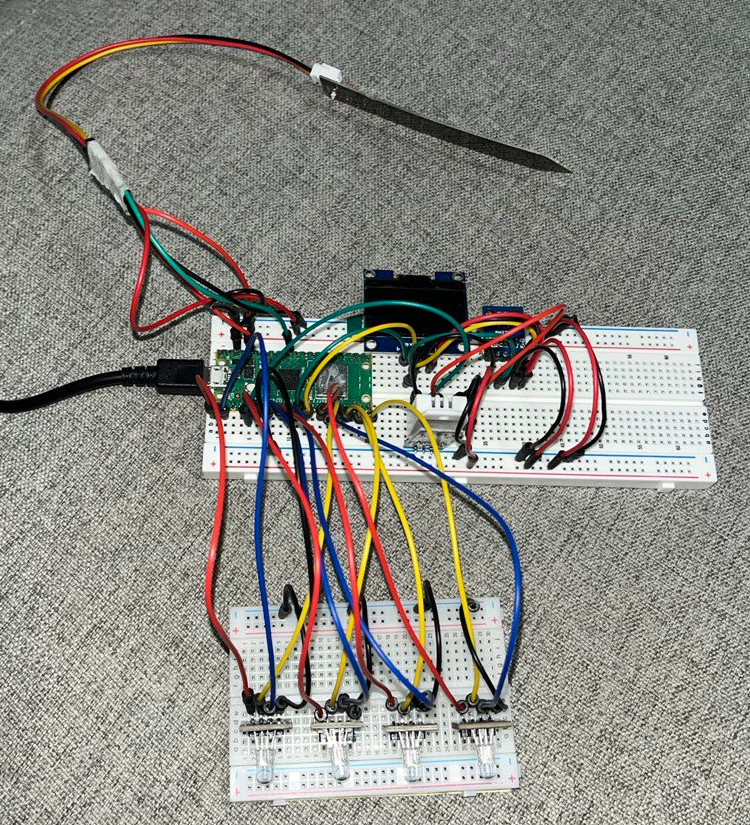
\includegraphics[width=0.4\textwidth]{img/fotos/conexiones_real.png}
	\caption{Raspberry Pi Pico W y sensores conectados mediante un protoboard.} \label{Img:conexion_simple}
\end{figure}

Una vez definida la idea del TFG y los componentes hardware, surgía la interrogante: "¿Dónde enviar los datos? ¿Cómo gestionarlos?". La primera medida fue mostrar los datos en una pantalla OLED~\cite{manual:Oled} conectada a la protoboard.

\begin{figure}[h]
	\centering
	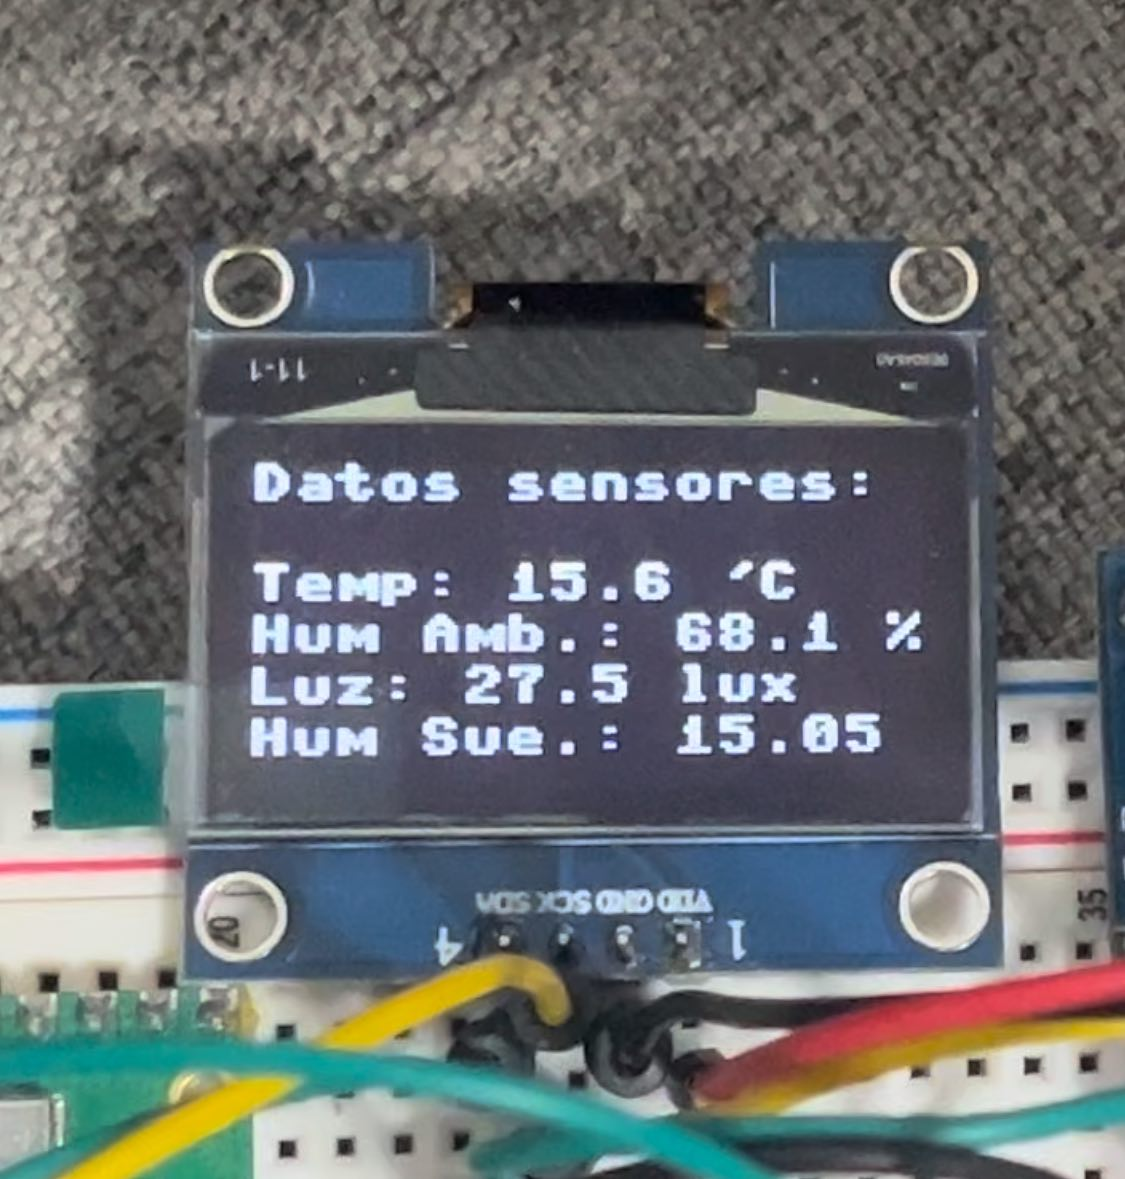
\includegraphics[width=0.4\textwidth]{img/fotos/oled1.png}
	\caption{Pantalla oled conectada a la Raspberry Pi Pico W.} \label{Img:oled_conexion}
\end{figure}

Sin embargo, al estar fuera de la red, surgieron nuevas incógnitas, ya que inicialmente se trató de un sistema unidireccional en el cual el sensor recolecta los datos y los muestra en la pantalla OLED.

Más tarde, se implementó la funcionalidad de enviar alertas a través de Telegram en caso de que los valores recopilados excedieran los umbrales ideales.

\begin{figure}[h]
	\centering
	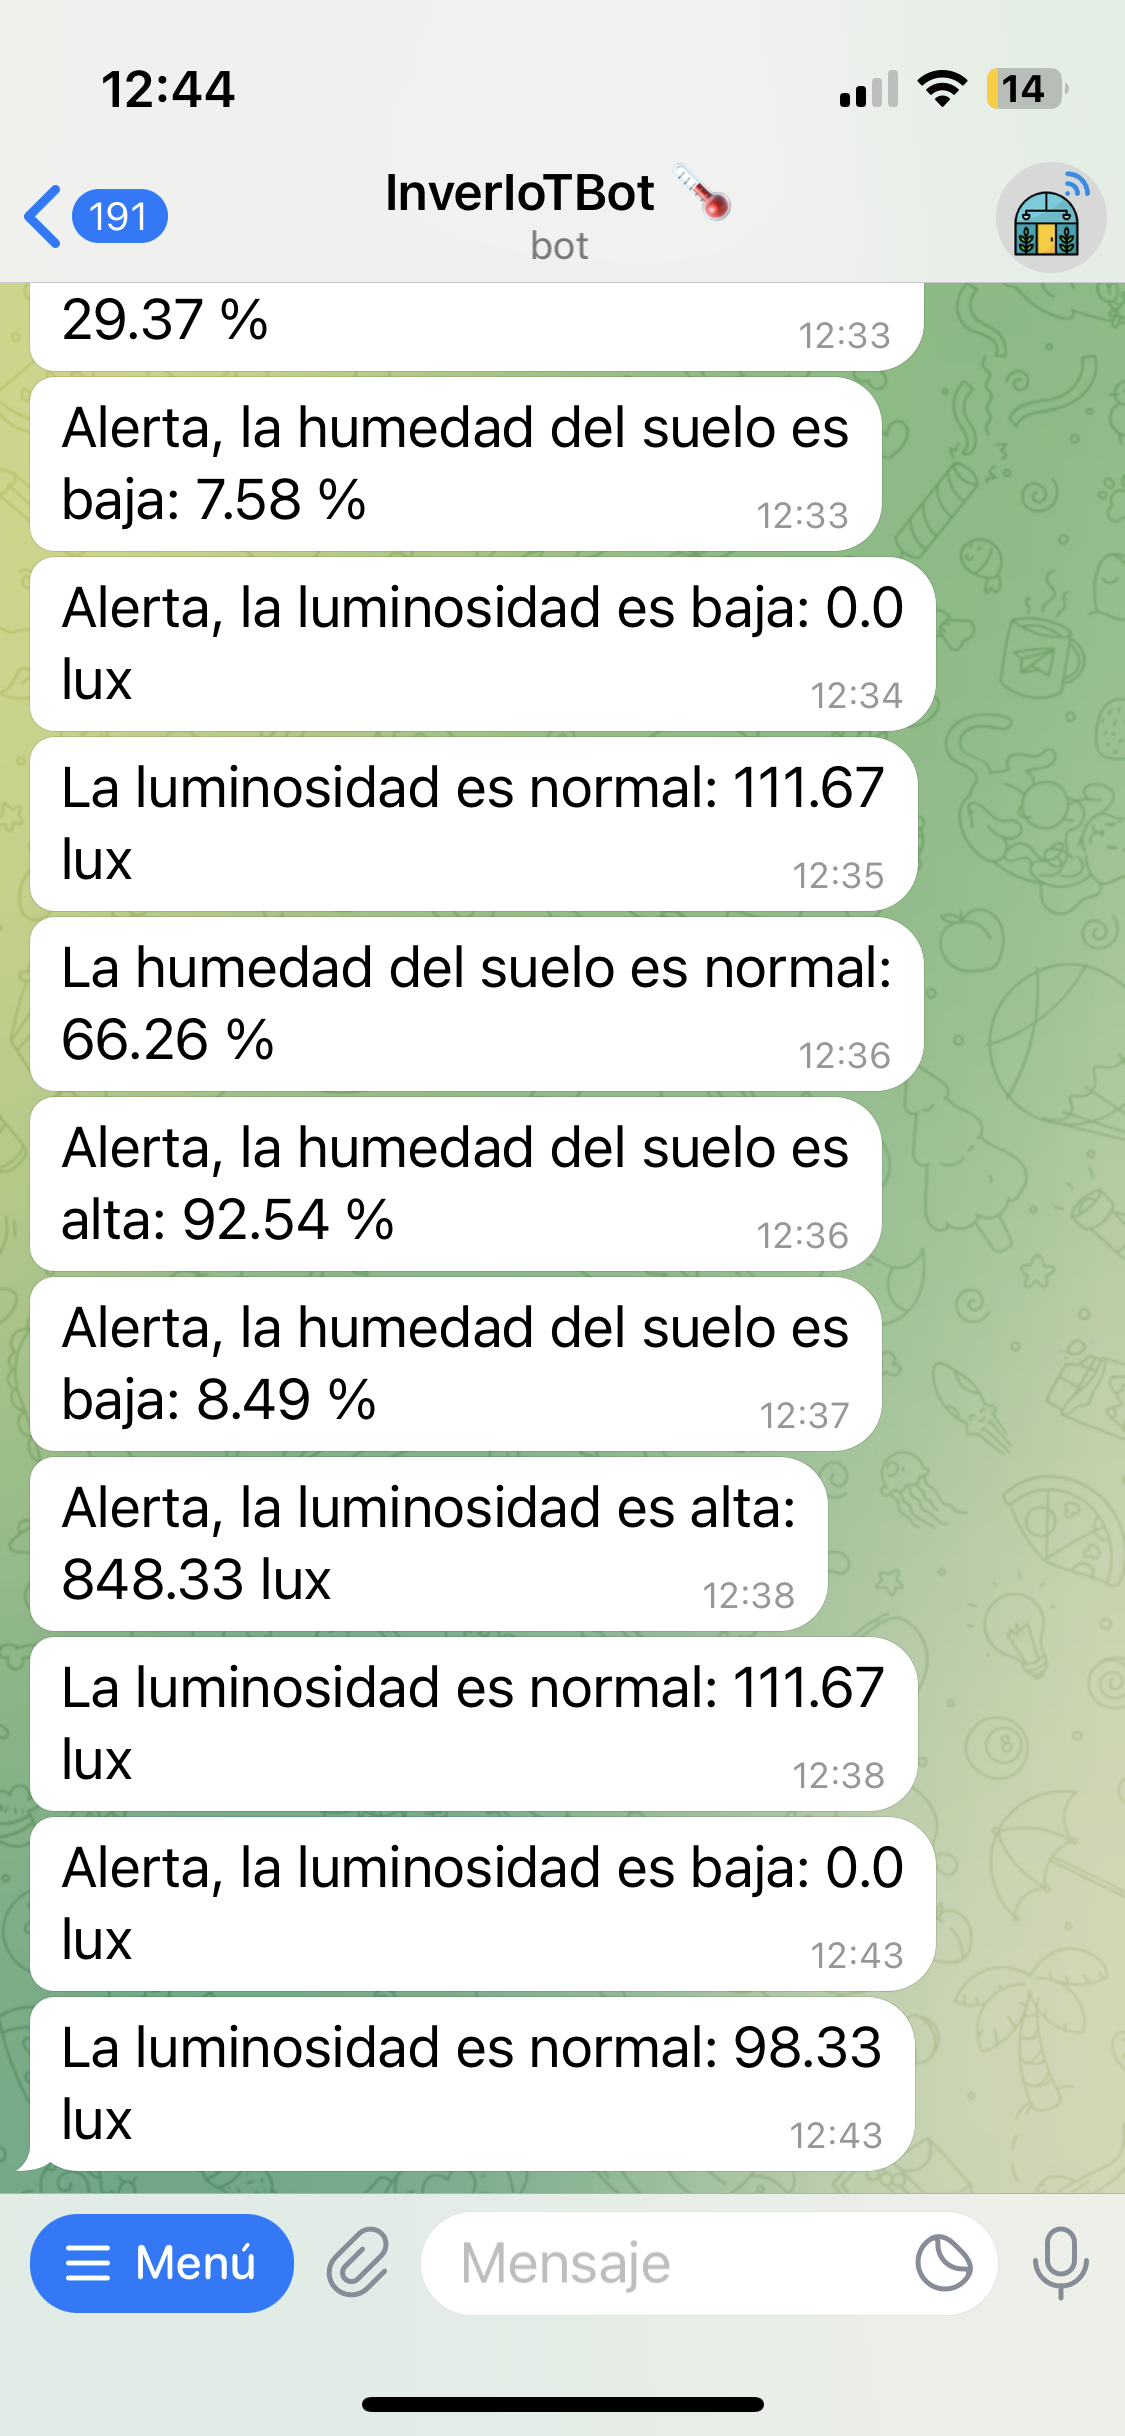
\includegraphics[width=0.27\textwidth]{img/desarrollo/BotTelegram_alertas.png}
	\caption{Alertas del bot de Telegram.} \label{Img:BotTelegram_alertas}
\end{figure}

Posteriormente, opté por establecer un servidor LAMP para facilitar el envío y manejo de datos. La implementación de este servidor se llevó a cabo en el sistema operativo Ubuntu~\cite{misc:Ubuntu}, el cual fue virtualizado utilizando Hyper-V~\cite{manual:Hyper_V}.
En esta instancia, se emplea un servidor físico HP ProLiant~\cite{misc:HP_ProLiant} para la virtualización de los servicios Apache~\cite{misc:Apache}, MySQL~\cite{misc:Mysql}, PHP~\cite{misc:PHP} y SSH~\cite{misc:SSH}.

\begin{table}[htbp]
\begin{center}
\caption{Características del servidor HP ProLiant.}
\begin{tabular}{|l|l|}
\hline
\rowcolor[HTML]{C0C0C0} 
\textbf{Característica} & \textbf{Descripción}\\ \hline
Sistema operativo & Windows Server 2019 Standard\\ \hline
Fabricante & Hewlett Packard Enterprise \\ \hline
Modelo & Hewlett Packard Enterprise x64 Class PC\\ \hline
Procesador & Intel(R) Xeon(R) Silver 4210R CPU @ 2.4GHz 2.39GHz\\ \hline
Memoria instalada (RAM) & 128 GB (128 GB utilizable) \\ \hline
Tipo de sistema & Sistema operativo de 64 bits, procesador x64 \\ \hline
\end{tabular}
\end{center}
\end{table}

\begin{figure}[h]
	\centering
	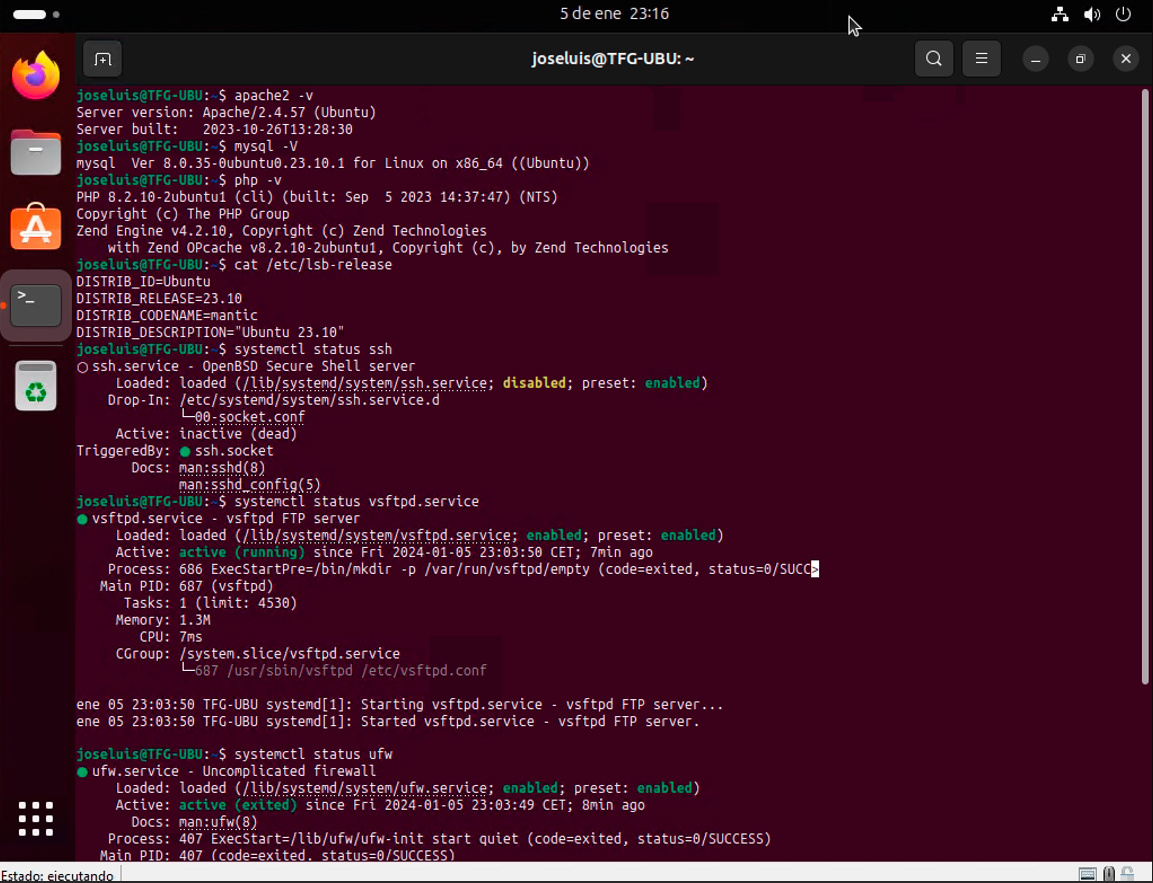
\includegraphics[width=1\textwidth]{img/desarrollo/LAMP_servicios.png}
	\caption{Servicios instalados y operativos en el servidor LAMP.} \label{Img:LAMP_servicios}
\end{figure}

Basándome en esta información y en mi experiencia previa trabajando con \textbf{Smart Cities}, tomo la decisión de enviar la información recopilada por los sensores al servidor mediante MQTT~\cite{manual:MQTT}. 

\begin{figure}[h]
	\centering
	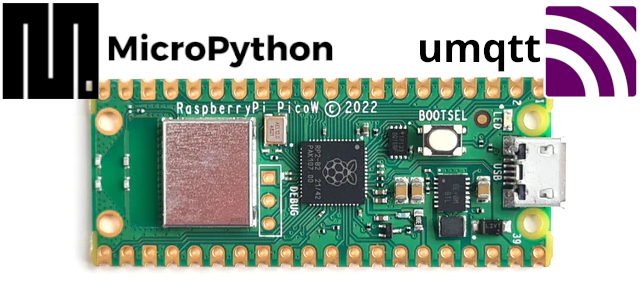
\includegraphics[width=0.7\textwidth]{img/herramientas/rpipicow_umqtt.png}
	\caption{Se ha implementado la libreria umqtt en la Raspberry Pi Pico W.} \label{Img:rpipicow_umqtt}
\end{figure}

MQTT permite la visualización en tiempo real de los datos en una página web alojada en el servidor LAMP cada vez que la placa junto con el sensor envíe datos. Además, posibilita el almacenamiento de los datos en la base de datos MySQL~\cite{misc:Mysql}, permitiéndome mantener un historial y realizar consultas. A esta parte del proyecto se ha llamado \textbf{NodeMqtt}~\ref{proyecto:NodeMqtt}.

\begin{figure}[h]
	\centering
	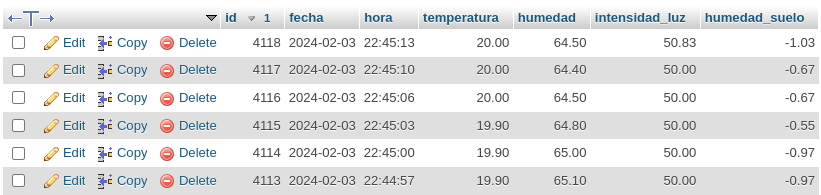
\includegraphics[width=1\textwidth]{img/desarrollo/mysql_data.png}
	\caption{Data almacenada en la base de datos.}
\end{figure}

Listo, he leído e incluso almacenado los datos que se envían. Además, con la implementación de un bot de Telegram~\cite{misc:Telegram}, ahora puedo consultar en tiempo real la información proveniente de los sensores.

\begin{figure}[h]
	\centering
	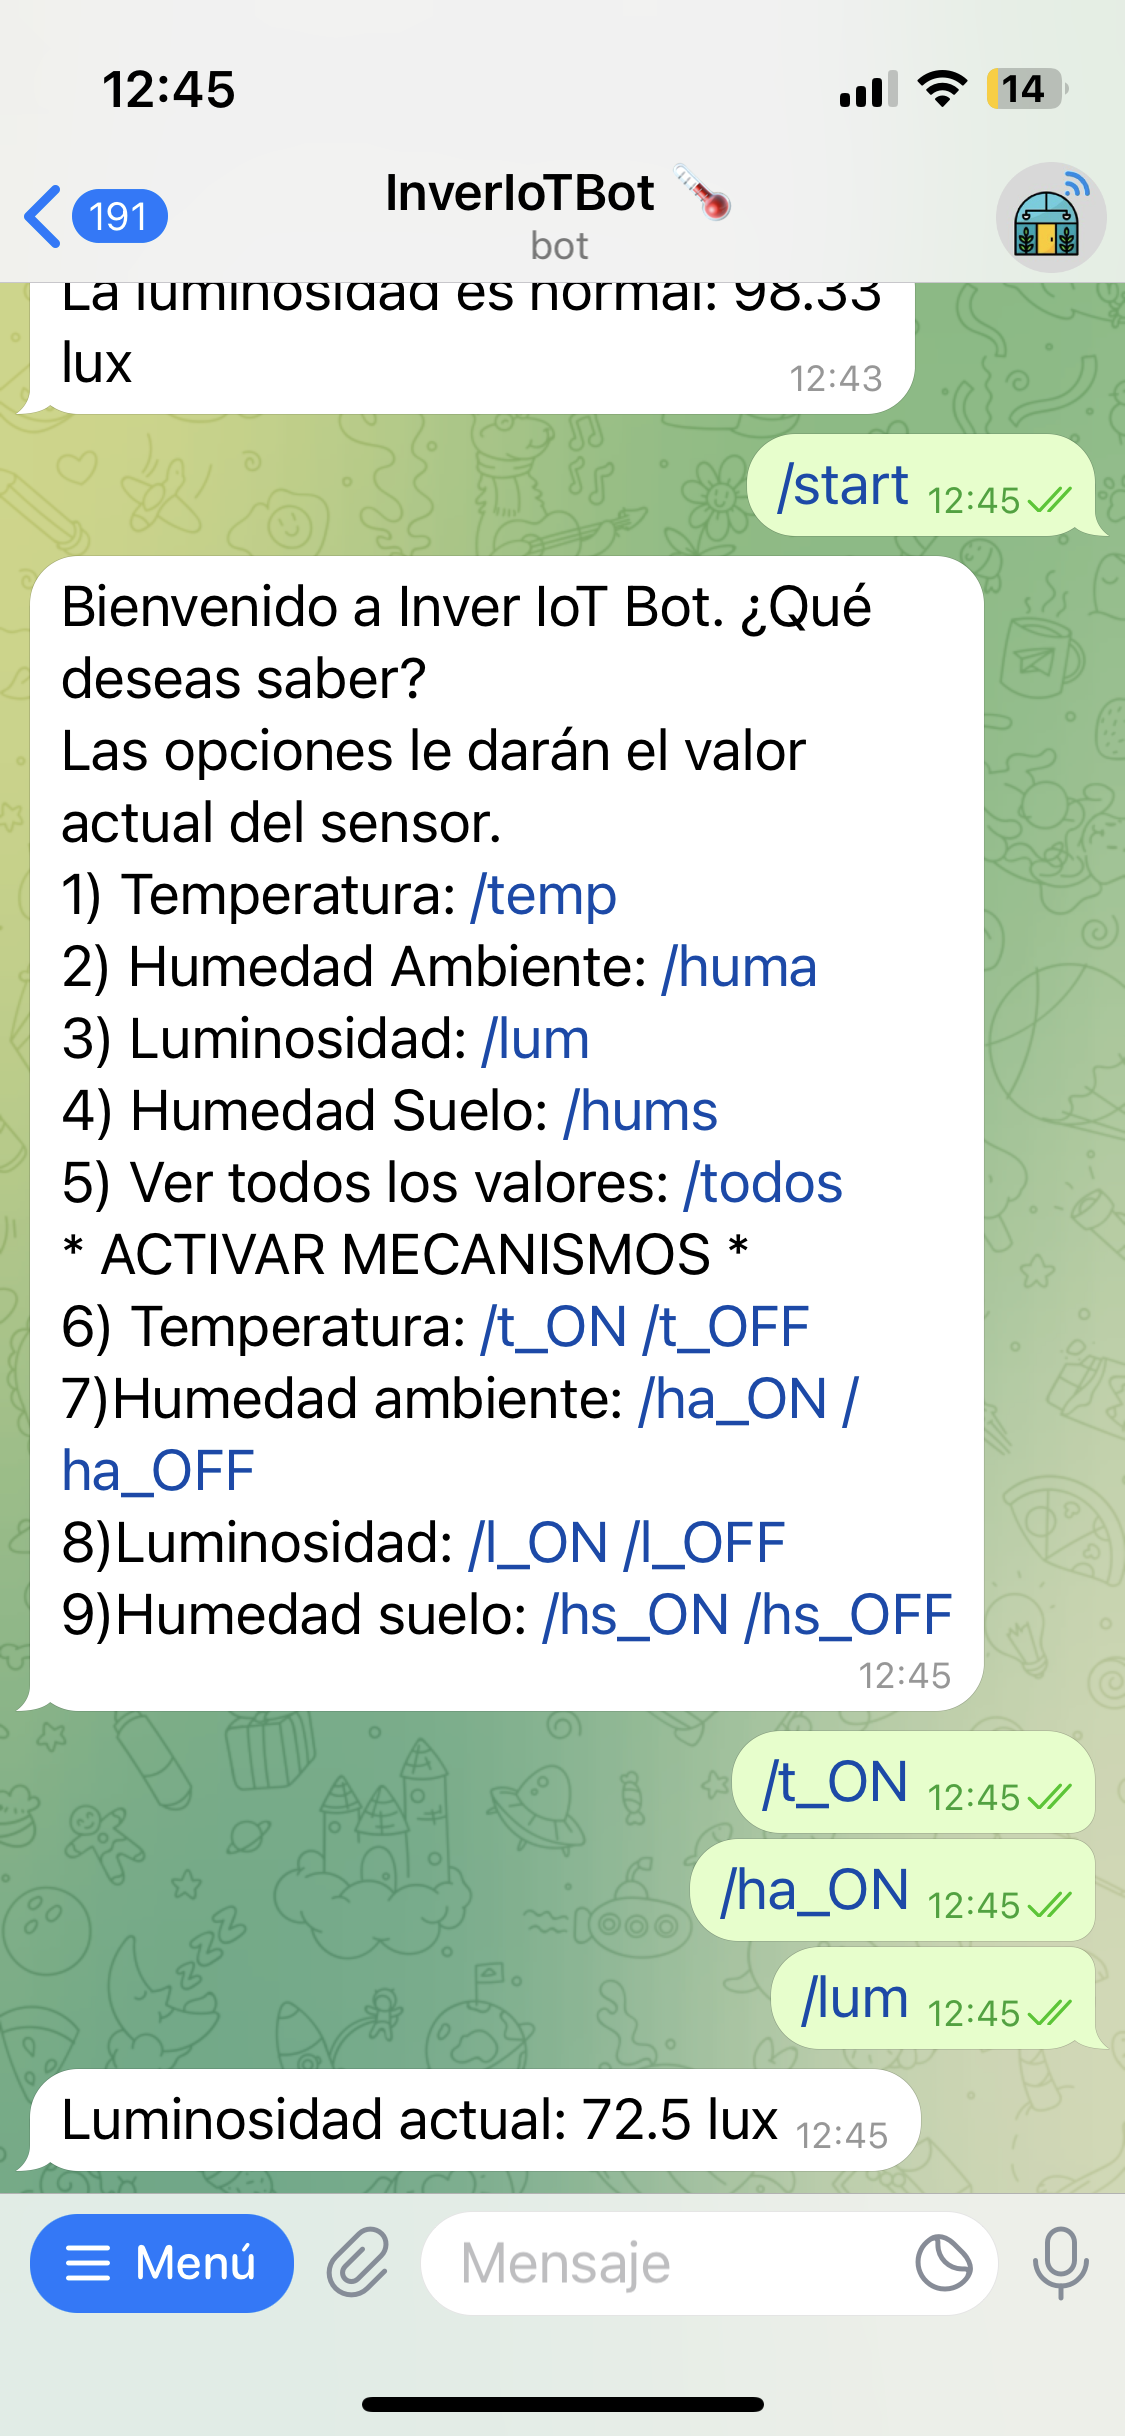
\includegraphics[width=0.32\textwidth]{img/desarrollo/BotTelegram_comandos.png}
	\caption{Consulta a la base de datos mediante comandos usando Telegram.}
\end{figure}

También optamos por desarrollar una aplicación de escritorio para Windows en C\#~\cite{manual:CSharp} al que se ha llamado \textbf{InverIoT}~\ref{proyecto:InverIoT}, que permite la visualización en tiempo real de los datos. ¡Problema resuelto! Ahora, puedo recibir y monitorear la temperatura, luminosidad y otros valores del invernadero.

\begin{figure}[h]
	\centering
	\includegraphics[width=0.61\textwidth]{img/fotos/InverIoT_PasandoUmbralLuz.png}
	\caption{El led rojo y el color naranja en la aplicación InverIoT indican que se ha sobrepasado el umbral de luz.}
\end{figure}

Sin embargo, al caer la noche, la luminosidad y la temperatura disminuyen, planteando un nuevo desafío. En este caso, necesitaría establecer una comunicación bidireccional con la placa Raspberry Pi Pico W para, por ejemplo, encender los focos y activar los calentadores.

Este cambio a una comunicación bidireccional se logró suscribiendo la Raspberry Pi Pico W a un topic MQTT. Ahora, puedo enviar órdenes para procesarlas según sea necesario. 

\begin{figure}[h]
	\centering
	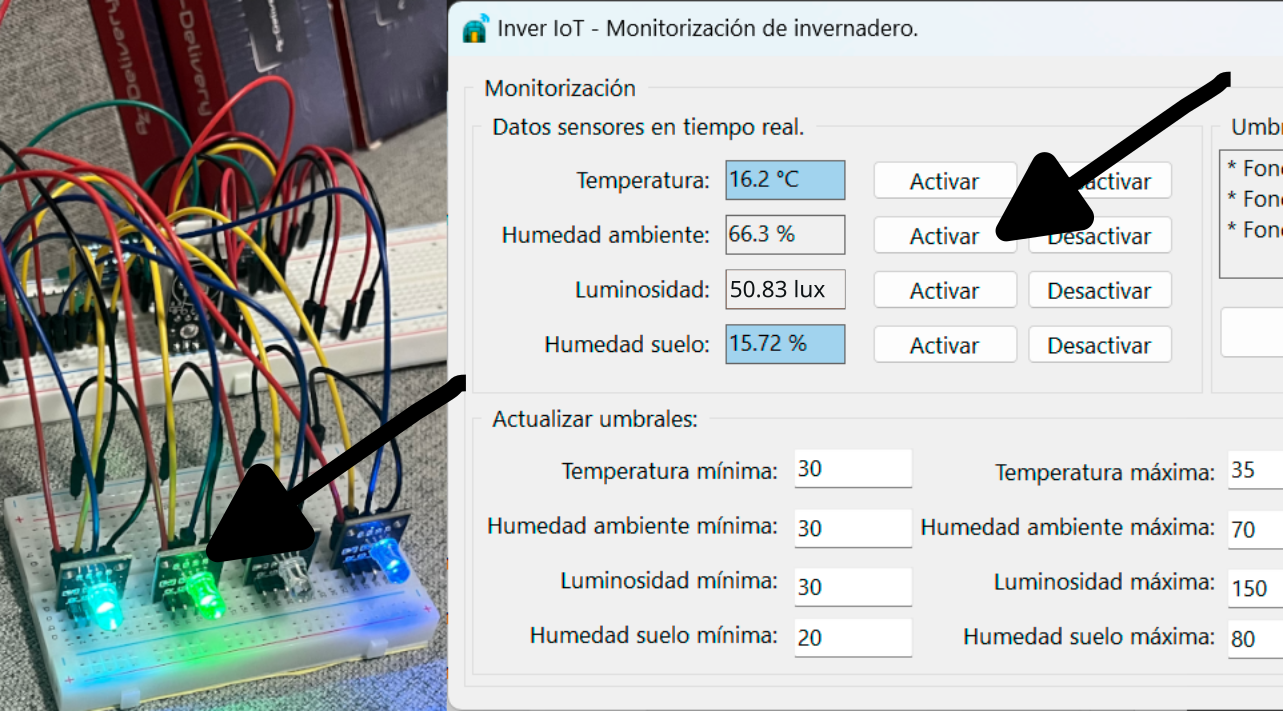
\includegraphics[width=0.61\textwidth]{img/desarrollo/InverIoT_verde_clickMecanismo.png}
	\caption{Al hacer clic en activar se enciende el led de color verde representando que estamos activando un mecanismo.}
\end{figure}

Sin embargo, la activación de mecanismos físicos como encender focos, activar calefacción, regar el suelo o humidificar el ambiente aún no se ha implementado, ya que corresponde a otras especialidades como telecomunicación industrial o mecánica.

El cannabis medicinal requiere condiciones ambientales constantes y dentro de un umbral específico para un crecimiento óptimo y delicado.

Definimos umbrales (valor mínimo/máximo) para mantener los valores de los sensores dentro de límites aceptables. En caso de detectar un valor anómalo fuera de estos umbrales, se genera una alerta. Para esta función, empleamos un bot de Telegram que envía mensajes de alerta, y se configura un LED RGB para cada medición (temperatura, humedad, luminosidad, humedad del suelo). Si la temperatura es baja, por ejemplo, el LED se ilumina en azul y envía una alerta por Telegram; si la temperatura es alta, el LED se enciende en rojo. Un LED apagado indica valores normales dentro del umbral.

\begin{table}[htbp]
\begin{center}
\caption{Umbrales ideales para un invernadero de cannabis medicinal.}
\begin{tabular}{|l|l|l|}
\hline
\rowcolor[HTML]{C0C0C0} 
\textbf{Característica} & \textbf{Mínimo} & \textbf{Máximo} \\ \hline
TEMPERATURA & 30 & 35\\ \hline
HUMEDAD & 30 & 70\\ \hline
LUMINOSIDAD & 30 & 150\\ \hline
HUMEDAD DEL SUELO & 20 & 80\\ \hline
\end{tabular}
\end{center}
\end{table}

La intervención manual también es posible, como activar ventiladores al observar un LED azul. Además, estos procesos pueden automatizarse. Por ejemplo, si la luminosidad cae por debajo del umbral, los focos se encienden hasta alcanzar el valor óptimo, por ahora eso no está implementado en este proyecto.

La información se visualiza en tiempo real en una página web desarrollada con Node.js, incluyendo un histórico de datos almacenados en la base de datos.

\begin{figure}[h]
	\centering
	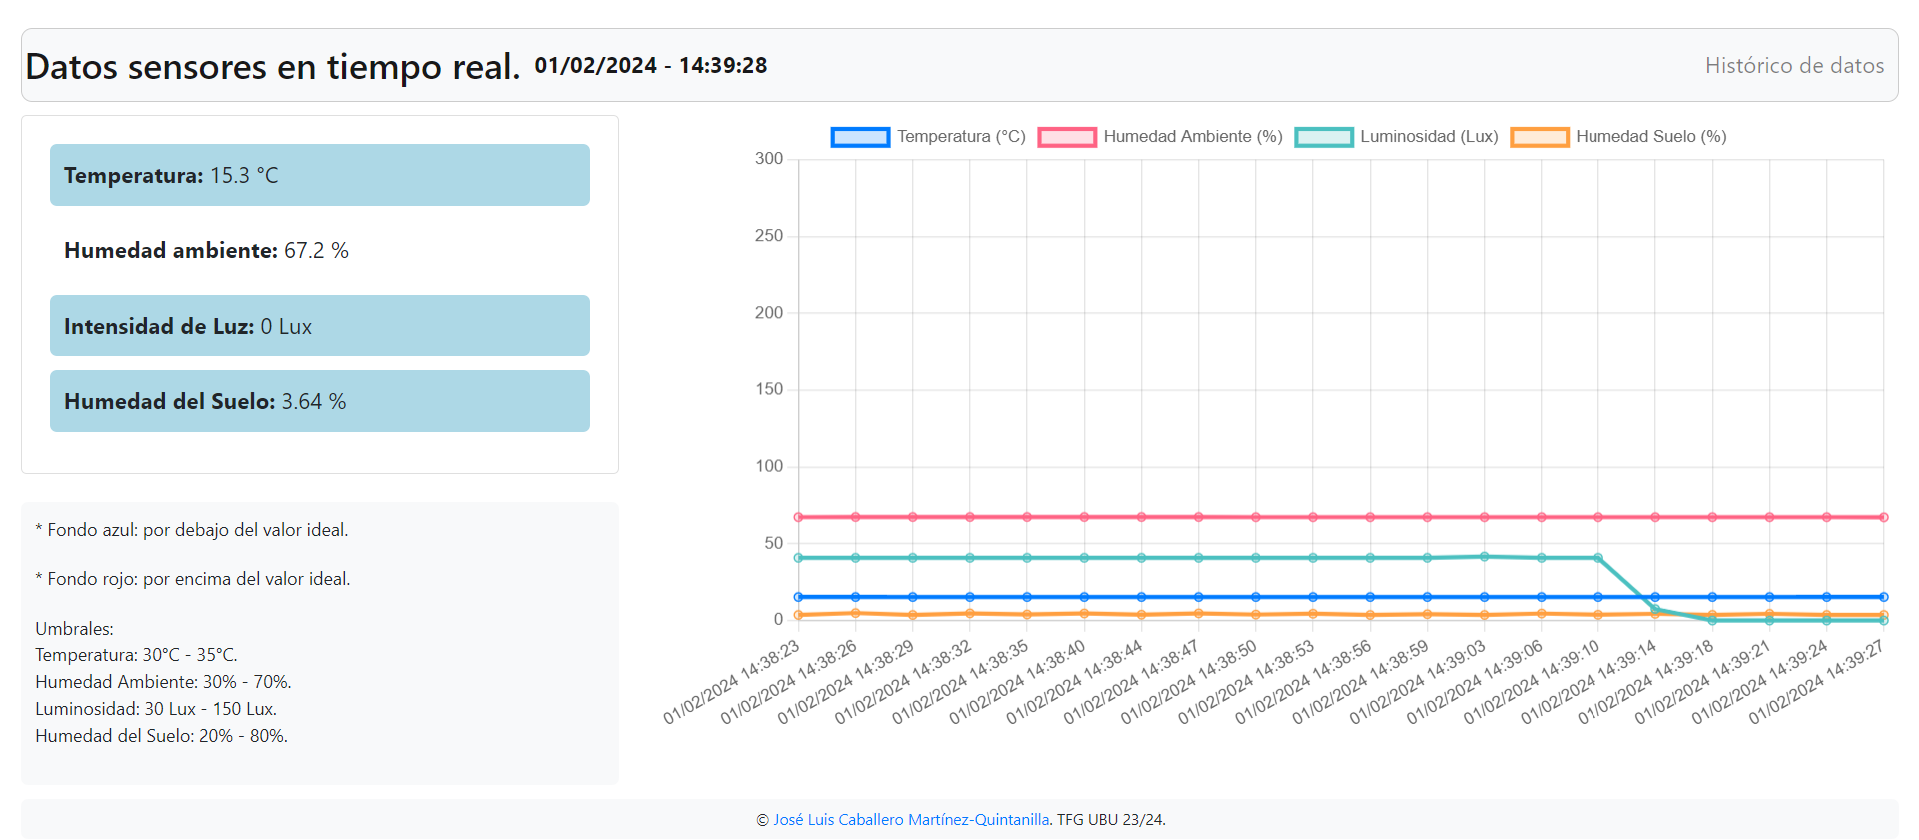
\includegraphics[width=0.9\textwidth]{img/desarrollo/Dashboard3.png}
	\caption{Página Web \href{http://www.inveriot.com}{InverIoT} desarrollada con Node.js.}
\end{figure}

%En este contexto, detallaré la configuración del servidor y la implementación de Node.js en la página web.

\subsection{Hardware}\label{proyecto:Hardware}
\begin{itemize}
	\item La Raspberry Pi Pico W estará situada en el invernadero para la recopilación de datos.
	\item Los LEDs RGB, instalados en la oficina del cliente, indicarán visualmente si los valores superan los umbrales establecidos.
	\item La pantalla OLED estará colocada en la puerta del invernadero para mostrar los valores actualizados.
\end{itemize}

\begin{figure}[h]
    \centering
    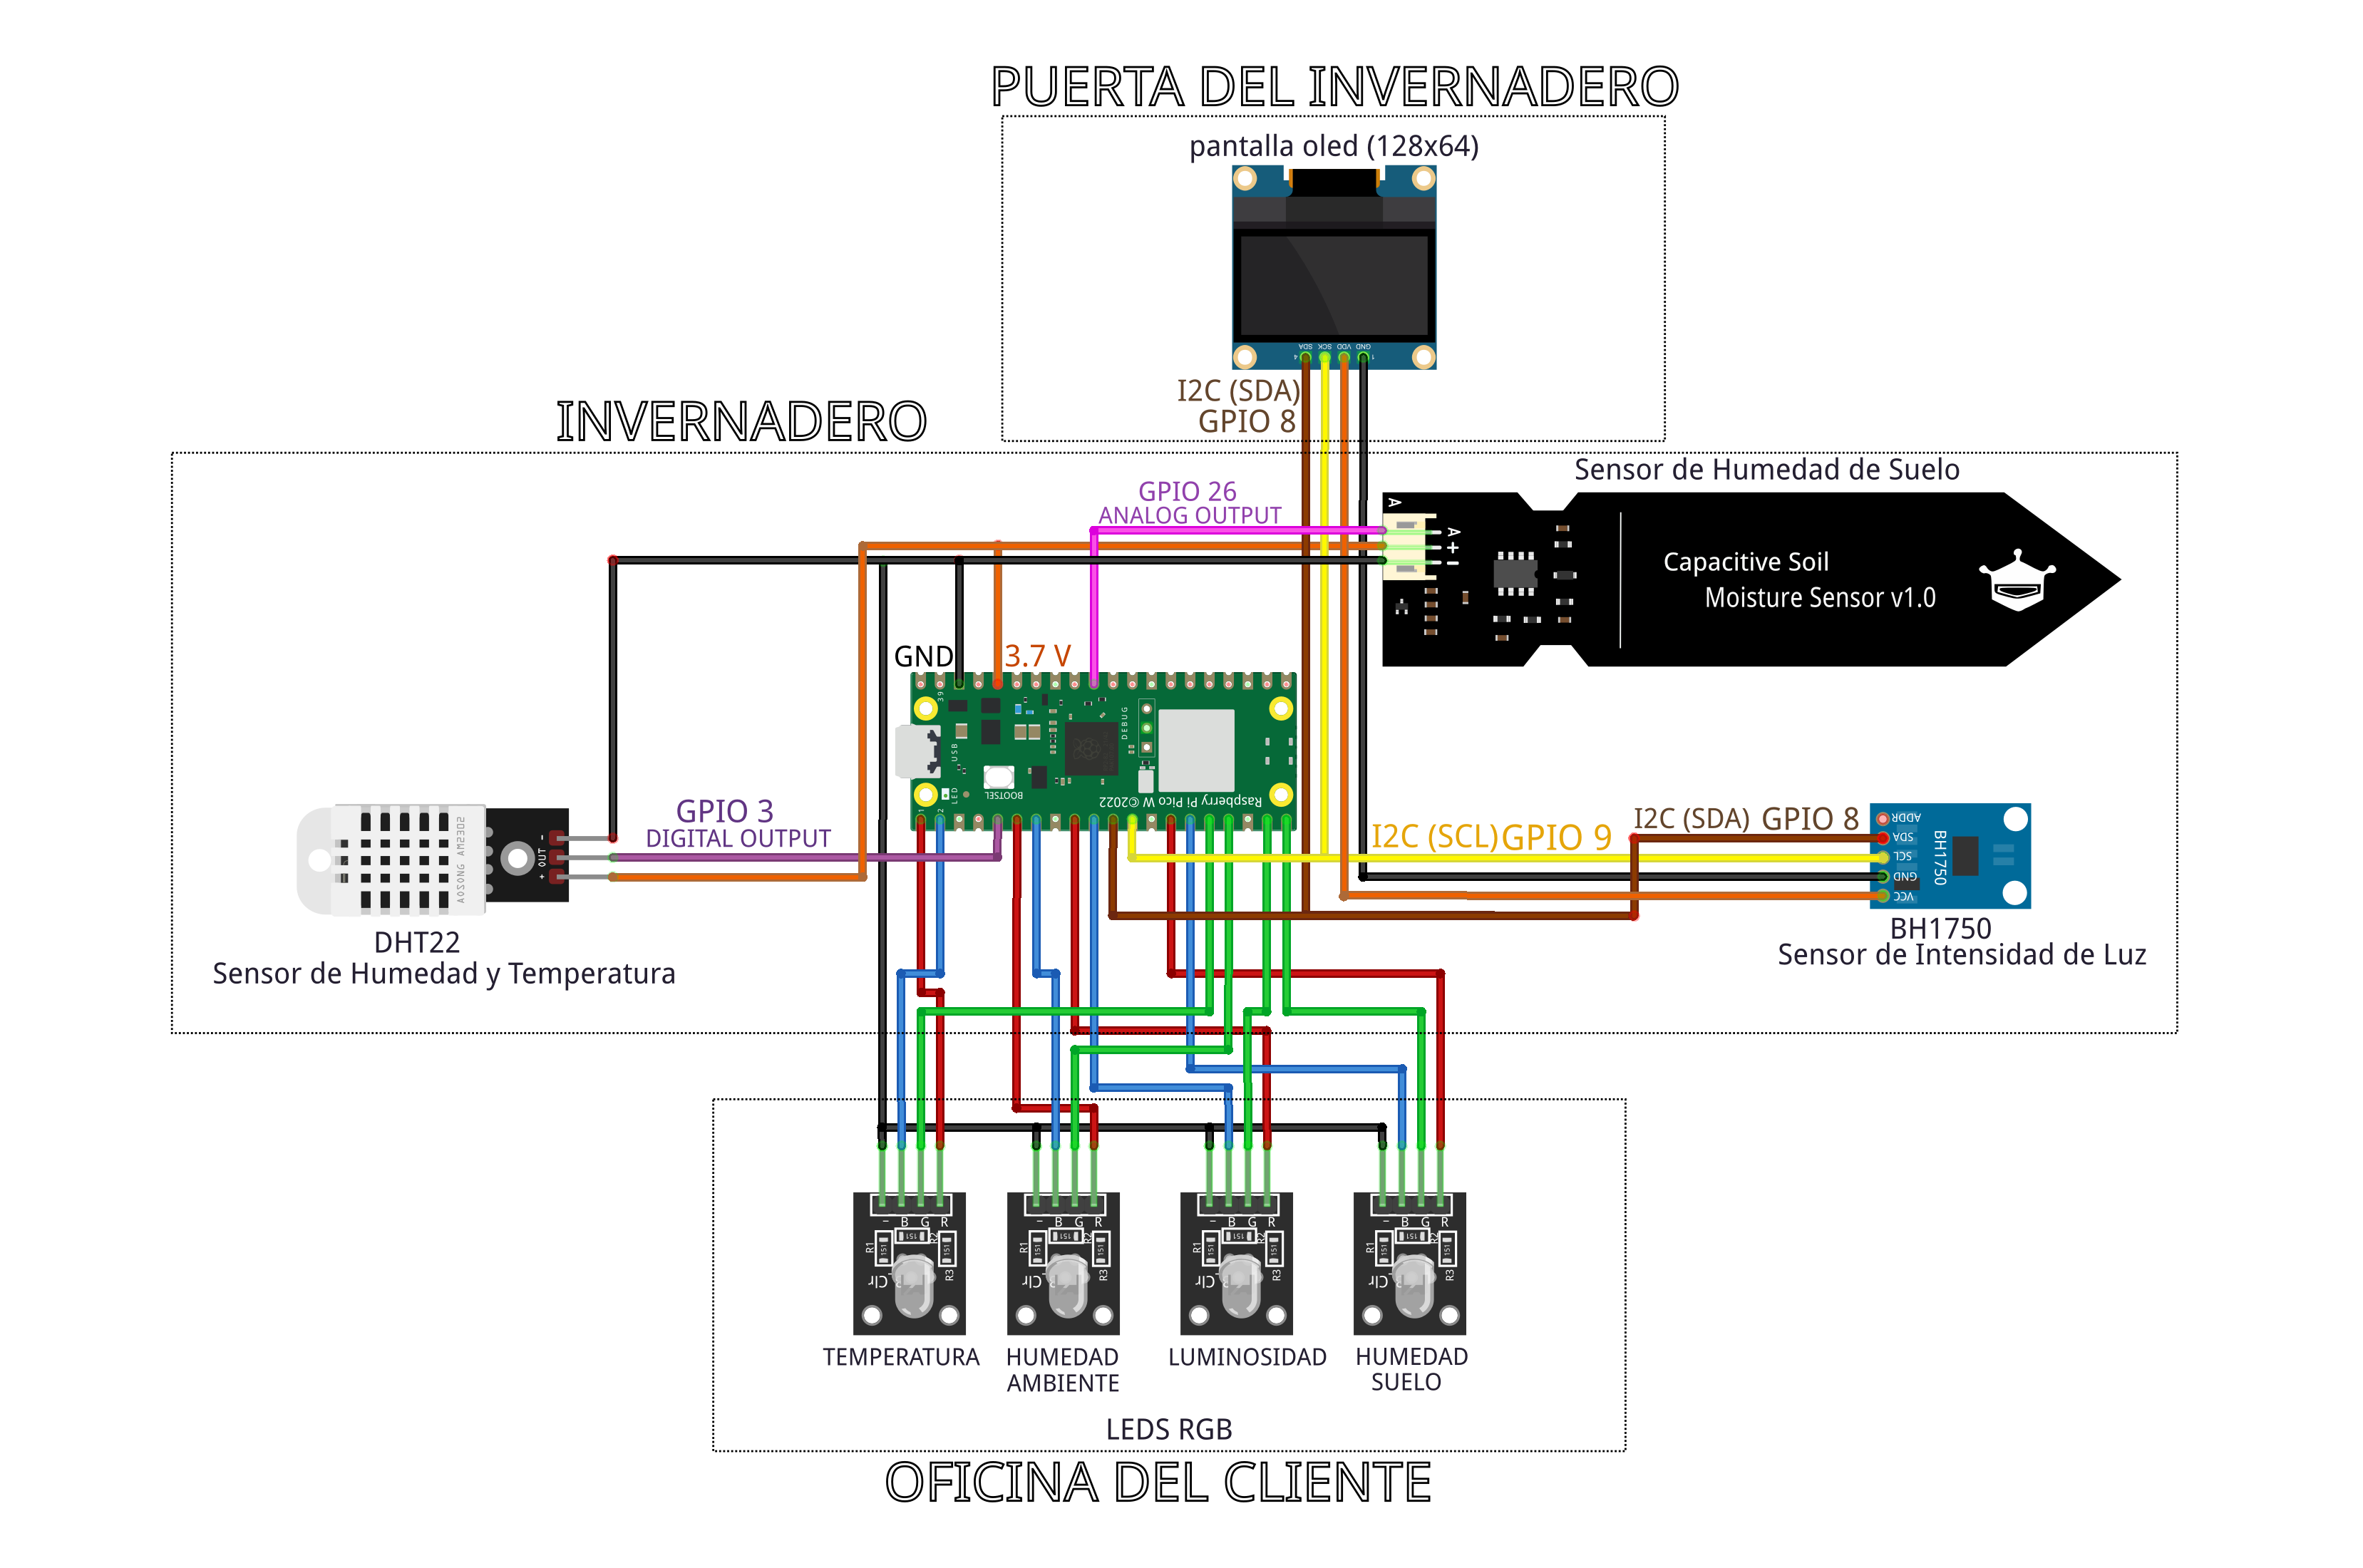
\includegraphics[width=1\textwidth]{img/diagramas/conexiones.png}
    \caption{Conexiones.} \label{Img:conexionesHardware}
\end{figure}
\pagebreak

\subsection{InverIoT}\label{proyecto:InverIoT}
Se desarrolla una aplicación de escritorio para Windows llamada InverIoT, que permite al usuario monitorizar en tiempo real los datos provenientes de los sensores conectados a la placa. 

\begin{figure}[h]
    \centering
    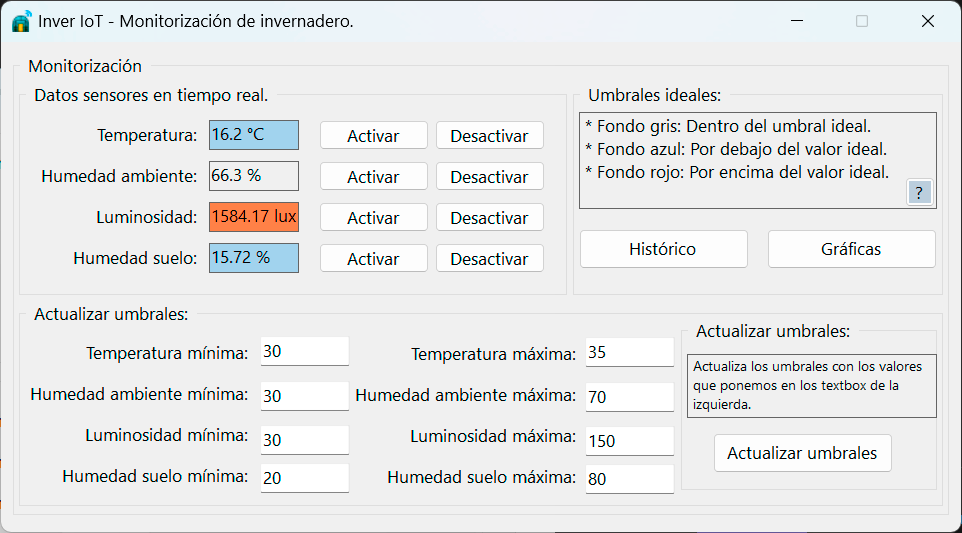
\includegraphics[width=0.95\textwidth]{img/desarrollo/InverIoT_Desktop.png}
	\caption{Aplicación de escritorio \textbf{InverIoT}.}
\end{figure}

Utilizando el protocolo MQTT~\cite{manual:MQTT}, la aplicación suscribe y recibe los datos publicados en el mismo tema. 

\begin{figure}[h]
    \centering
    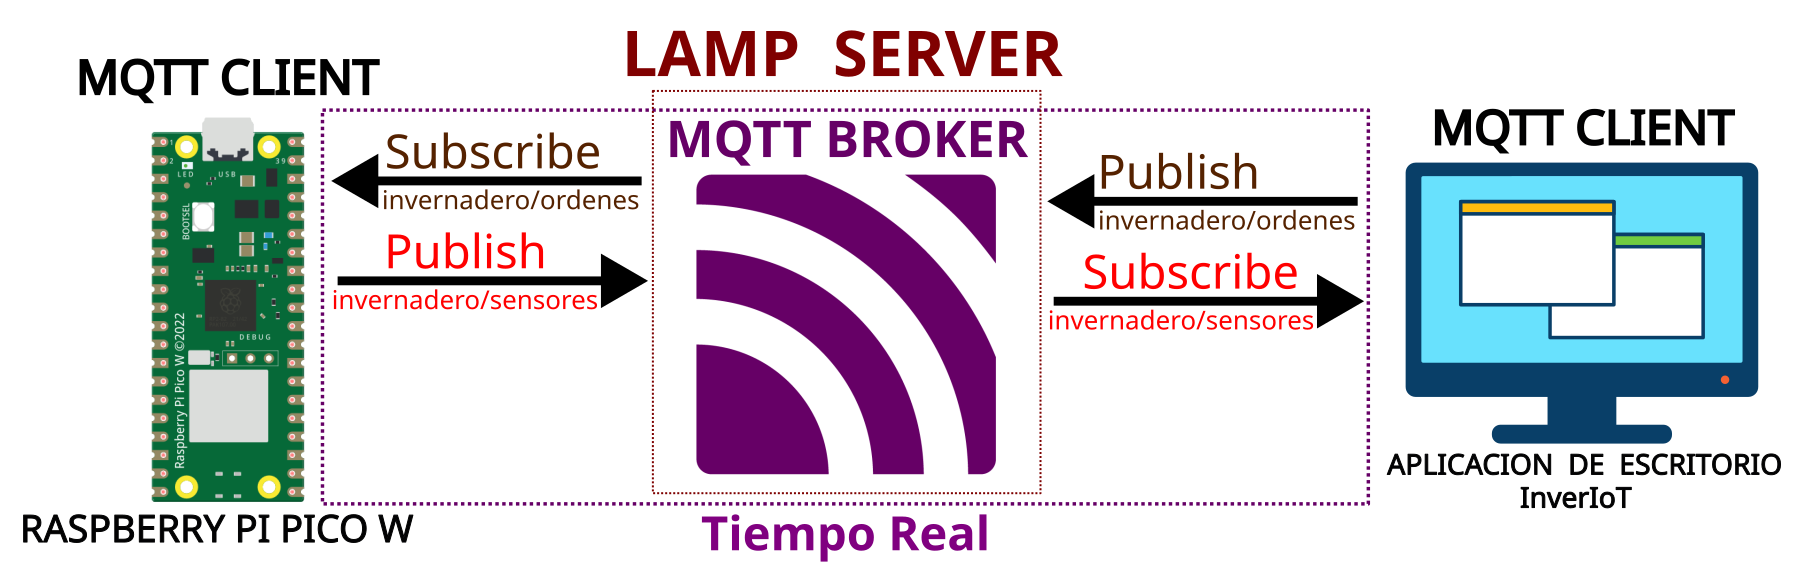
\includegraphics[width=0.95\textwidth]{img/diagramas/mqtt_InverIoT_TiempoReal.png}
    \caption{Enviando órdenes mediante MQTT la aplicación recibe datos en tiempo real.}
\end{figure}

\begin{figure}[h]
    \centering
    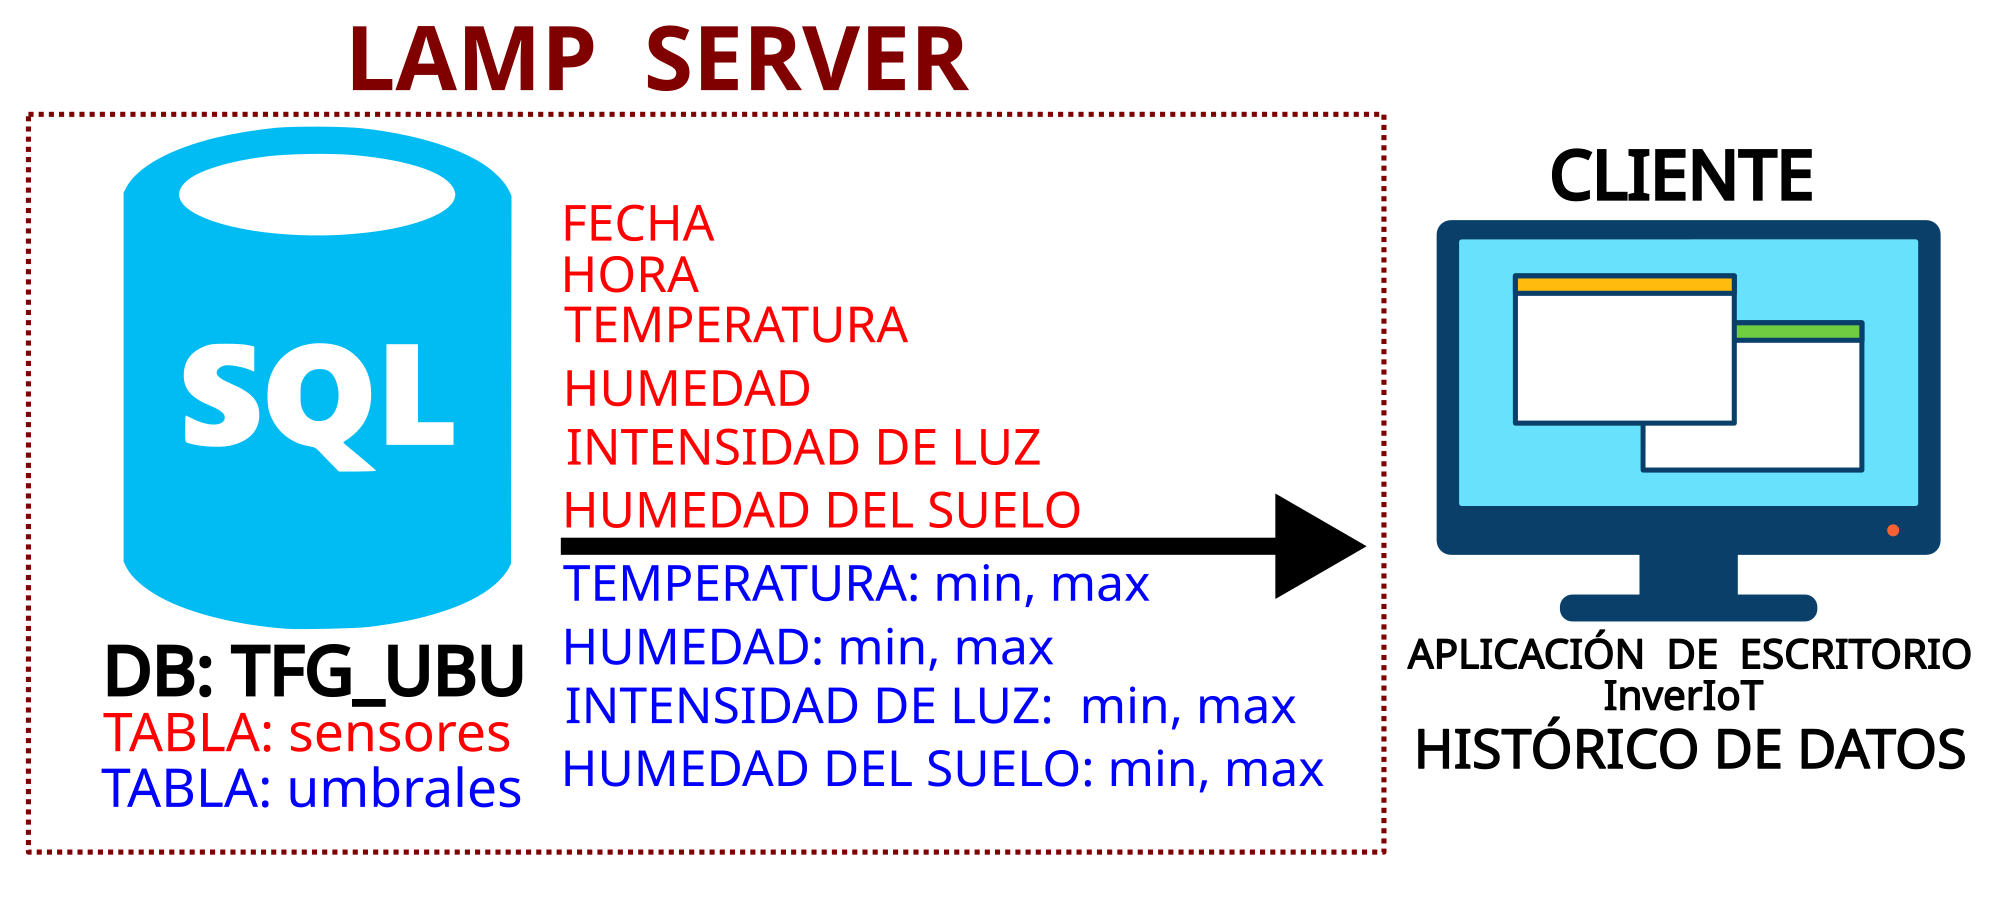
\includegraphics[width=1\textwidth]{img/diagramas/mqtt_InverIoT_Historico.png}
    \caption{Para mostrar el historial de datos la aplicación extrae información de una base de datos almacenada en un servidor LAMP.}
\end{figure}


Estos datos son formateados y presentados en textboxes correspondientes, con unidades de medida agregadas.

Se incorporan botones para activar o desactivar mecanismos, como un LED verde, que corrigen valores fuera de los umbrales ideales indicados en la parte derecha de la interfaz.

\begin{figure}[h]
    \centering
    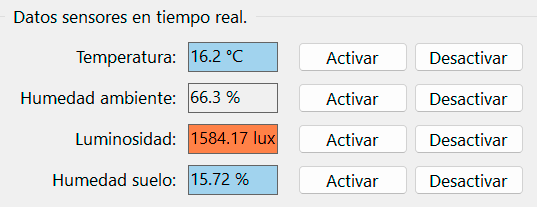
\includegraphics[width=1\textwidth]{img/desarrollo/InverIoT_Desktop_botones_control.png}
    \caption{Botones para activar o desactivar mecanismos.}
\end{figure}

Además, se añaden 8 textboxes en la parte inferior para ajustar manualmente los valores mínimos y máximos de cada parámetro.

Los umbrales se actualizan desde la base de datos del servidor LAMP, proporcionando indicadores visuales de color azul para valores bajos, gris para valores normales y rojo para valores altos.

Se desarrolló la aplicación de escritorio utilizando Windows Forms y programada en lenguaje \textbf{C\#}~\cite{manual:CSharp}.


La base de datos es alimentada por lo que en ese proyecto llamamos \textbf{NodeMqtt}~\ref{proyecto:NodeMqtt}, y la aplicación de escritorio \textbf{InverIoT} extrae esa información para mostrarla como un historial de datos.

La base de datos contiene dos tablas llamadas \textbf{sensores} y \textbf{umbrales}.

\begin{figure}[h]
    \centering
    \includegraphics[width=0.95\textwidth]{img/desarrollo/InverIoT_Histórico.png}
    \caption{Historial de los datos mostrara en la aplicación.}
\end{figure}


\begin{figure}[h]
    \centering
    \includegraphics[width=0.95\textwidth]{img/desarrollo/InverIoT_Gráficas.png}
    \caption{Gráfica mostrando los datos en un intervalo de fechas.}
\end{figure}
\pagebreak

\subsection{Dashboard}\label{proyecto:Dashboard}
Se desarrolla un dashboard que permite al usuario visualizar en tiempo real los datos capturados por los sensores, con una interfaz similar a la aplicación de escritorio.

Los valores que exceden los umbrales establecidos se destacan mediante cambios de color.

\begin{figure}[h]
    \centering
    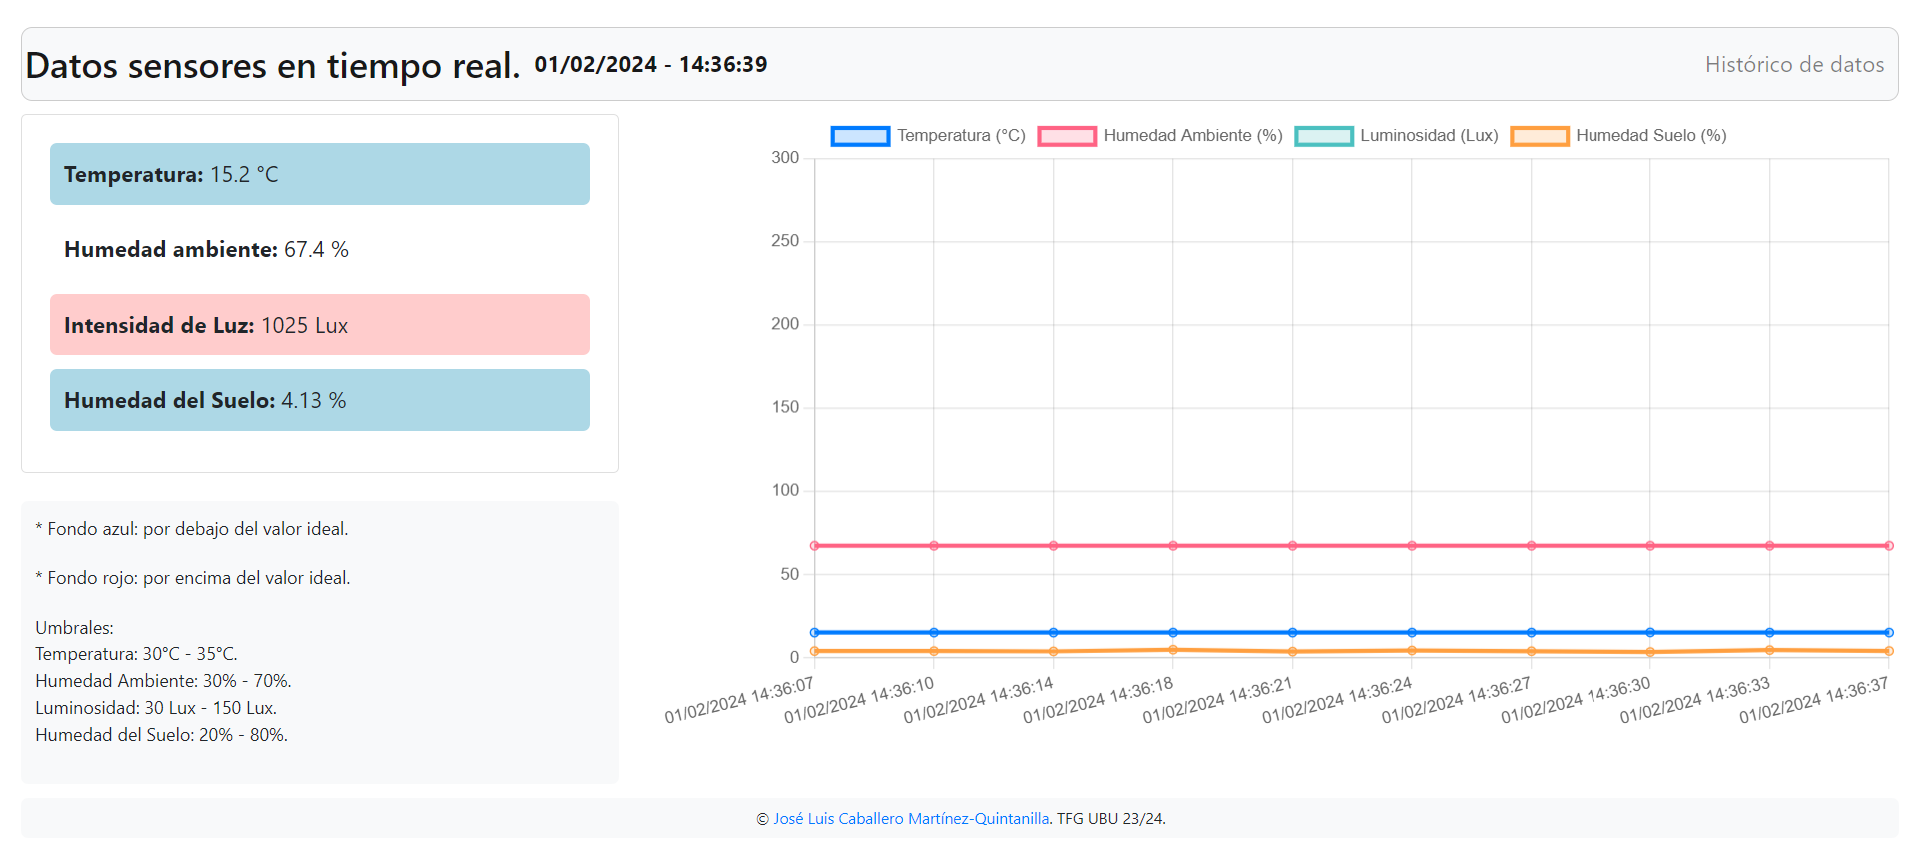
\includegraphics[width=0.95\textwidth]{img/desarrollo/Dashboard1.png}
    \caption{Intensidad de luz superando los umbrales.} \label{Img:Dashboard1}
\end{figure}

La plataforma incluye una gráfica en tiempo real y la capacidad de acceder a un historial con filtro de fecha.

\begin{figure}[h]
    \centering
    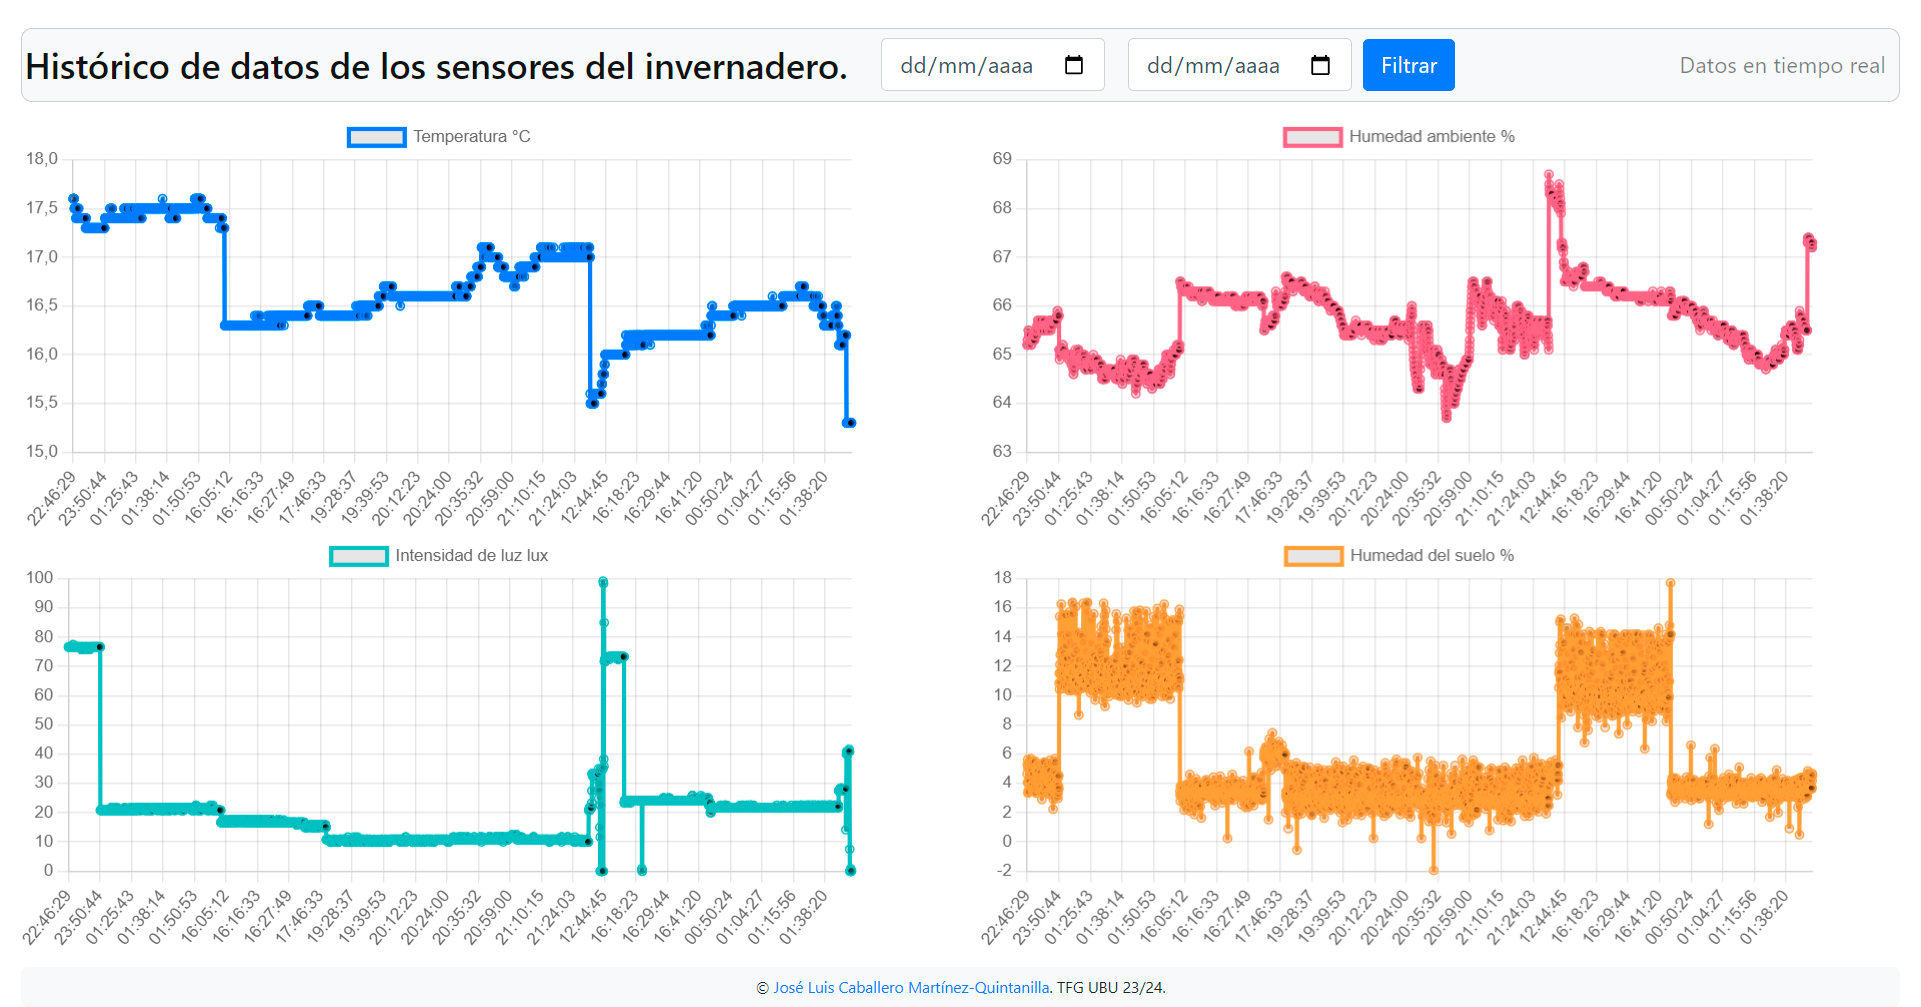
\includegraphics[width=0.95\textwidth]{img/desarrollo/Dashboard_Historico.png}
    \caption{Vista del historial, al cargar, muestra los datos del día actual.} \label{Img:Dashboard_Historico}
\end{figure}

Los umbrales utilizados se extraen de la tabla \textbf{TFG\_UBU} en la base de datos MySQL~\cite{misc:Mysql}.

\begin{figure}[h]
    \centering
    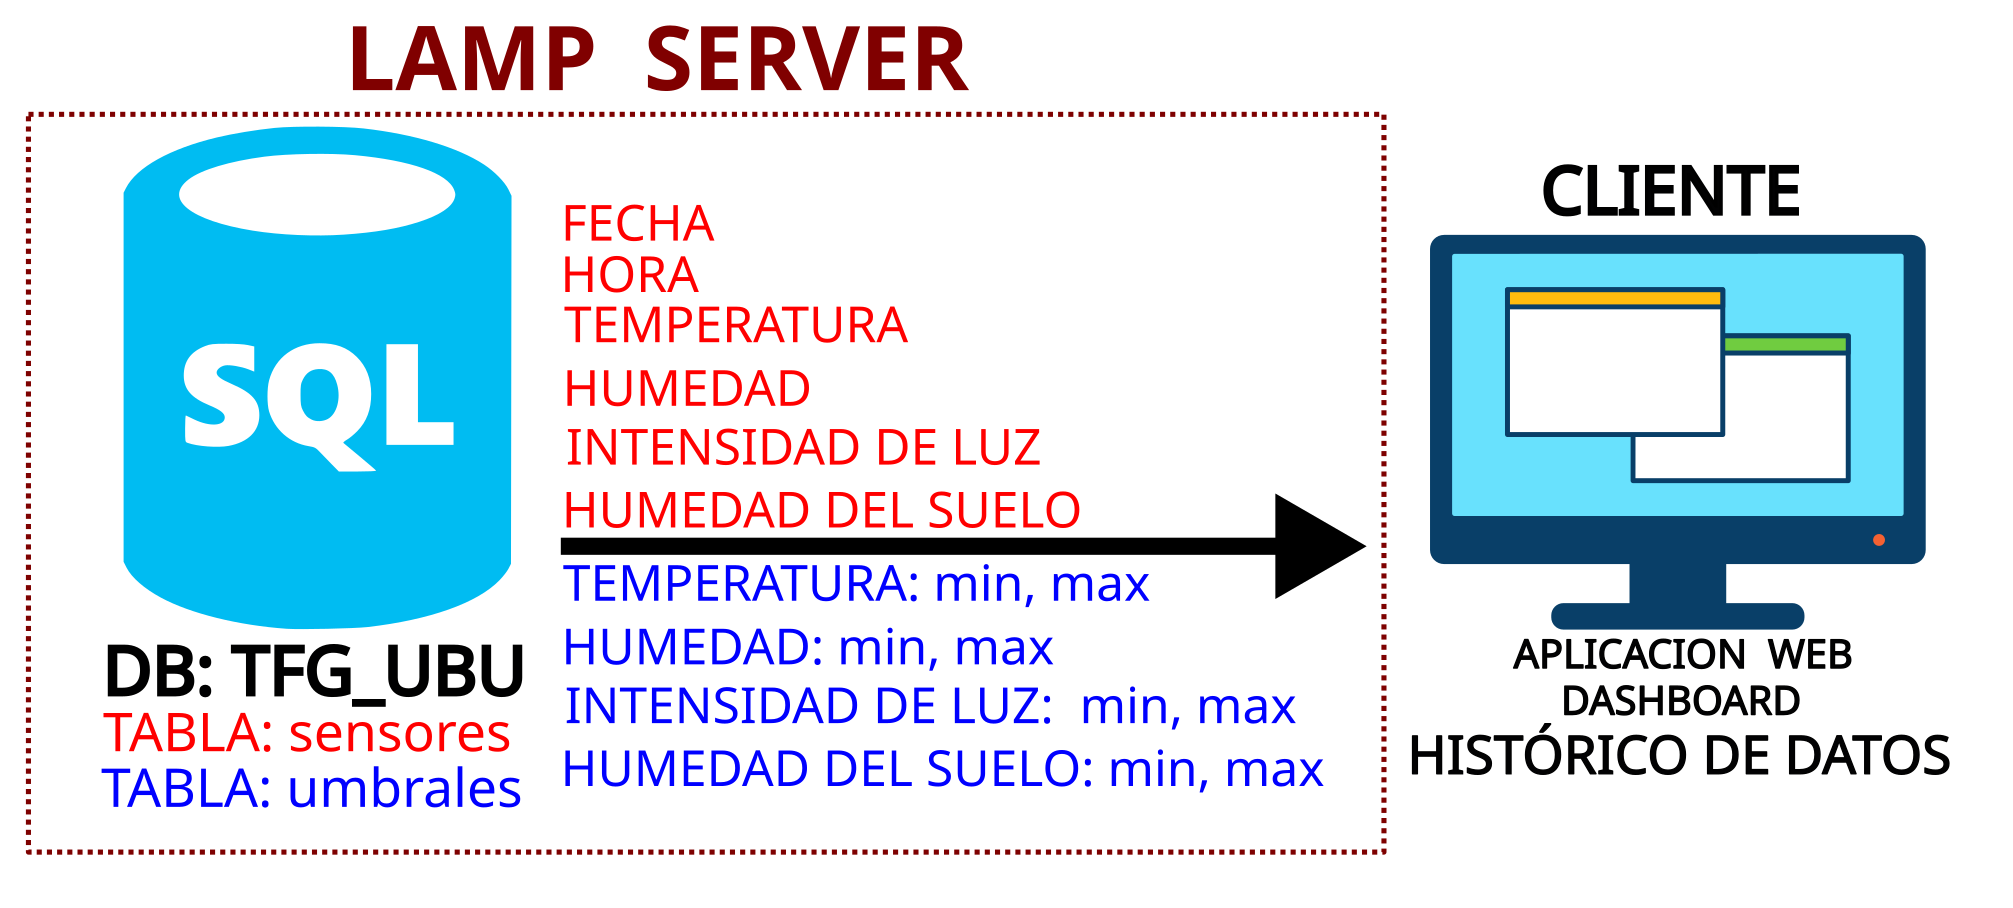
\includegraphics[width=1\textwidth]{img/diagramas/mqtt_dashboard_Historico.png}
    \caption{Extrae los datos de la base de datos para mostrar el historial.} \label{Img:Dashboard_diagrama_Historico}
\end{figure}

La Raspberry Pi Pico W utiliza una librería llamada \textbf{umqtt} para poder trabajar con MQTT, así es como envía data de los sensores y de los umbrales establecidos.

Los umbrales establecidos son almacenados en una base de datos que se encuentra en el servidor LAMP.

\begin{figure}[h]
    \centering
    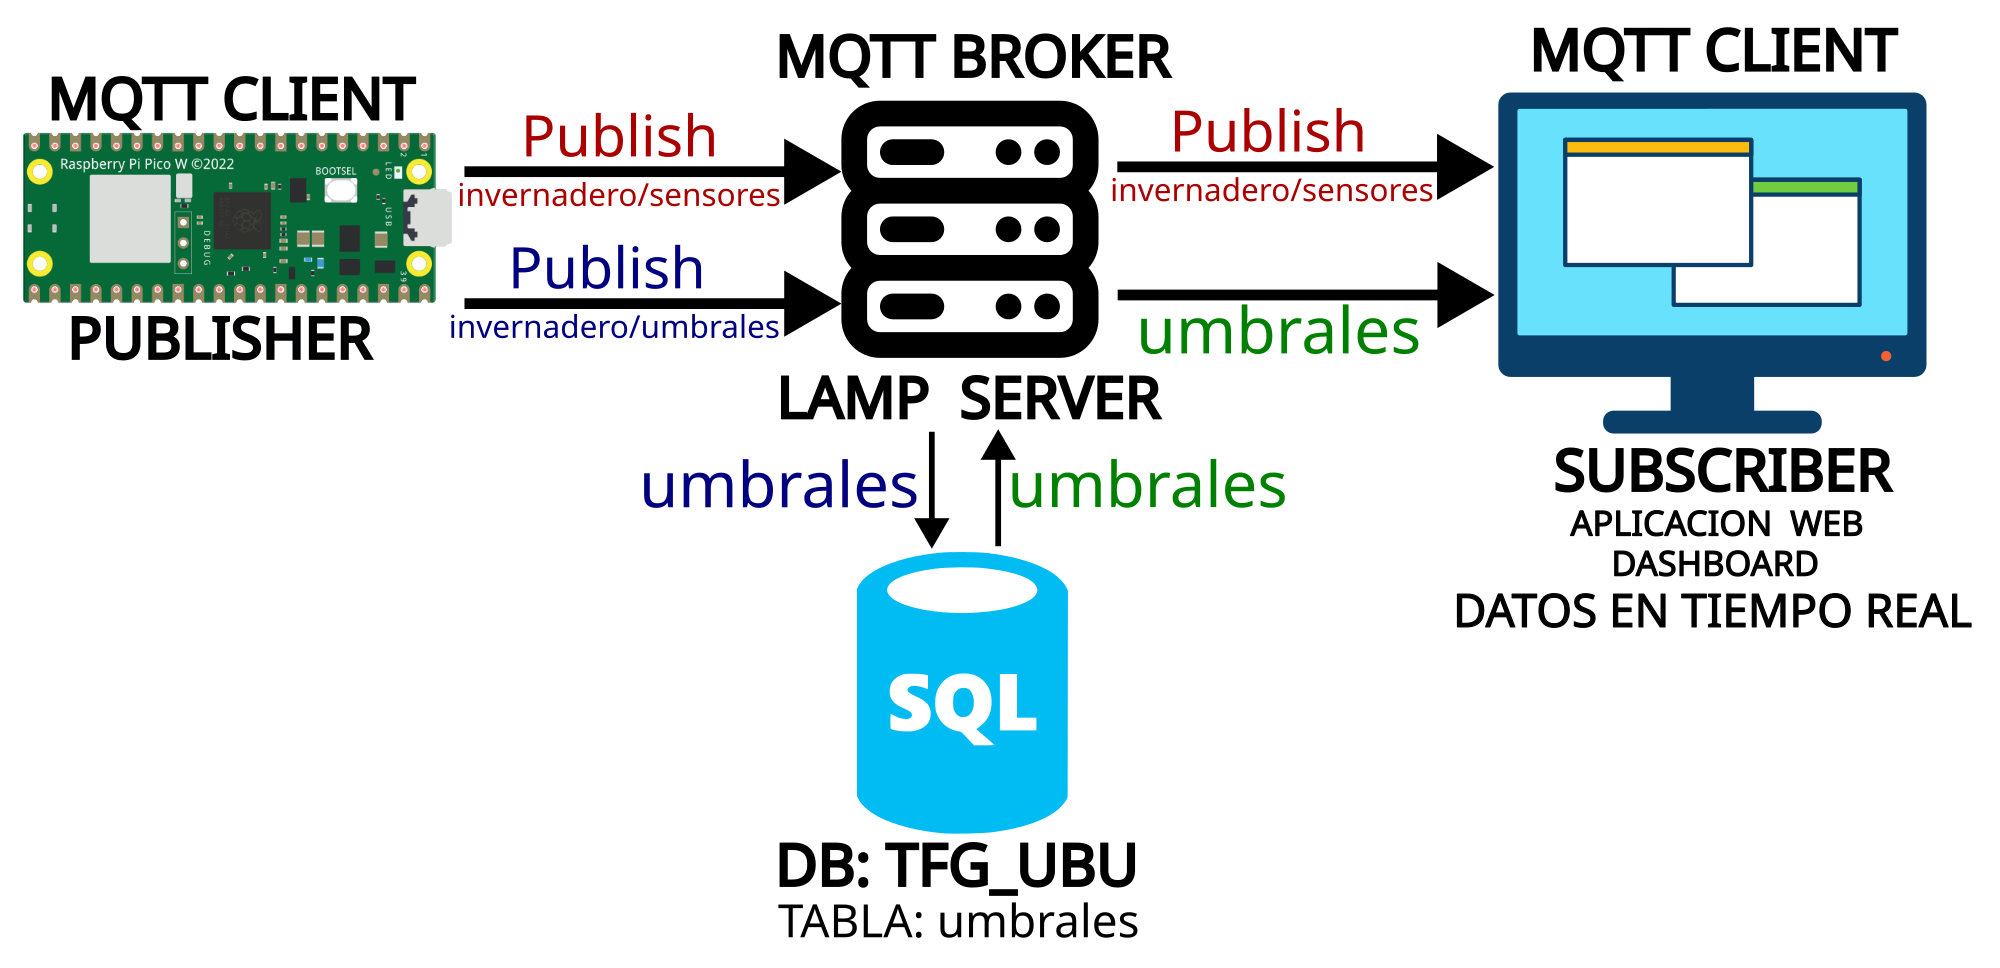
\includegraphics[width=1\textwidth]{img/diagramas/mqtt_dashboard_TiempoReal.png}
    \caption{Mediante MQTT extrae los datos para mostrarlos en tiempo real.} \label{Img:Dashboard_diagrama_TiempoReal}
\end{figure}

El panel de control está disponible para su acceso a través del siguiente enlace: \href{http://www.inveriot.com}{InverIoT Dashboard}



\subsection{NodeMqtt}\label{proyecto:NodeMqtt}
\textbf{nodeMqtt} es un servicio en Node.js~\cite{misc:Nodejs} que escucha los topics \textbf{invernadero/sensores} e \textbf{invernadero/umbrales}. Utiliza la librería MQTT.js~\cite{misc:MQTTjs}. Los datos son enviados por la placa Raspberry Pi Pico W RP2040~\cite{misc:RPiPicoW}, que recopila valores de sensores. El servicio \textbf{nodeMqtt} captura, formatea y luego inserta estos datos en la base de datos MySQL~\cite{misc:Mysql} para los valores de sensores, además de actualizar los umbrales correspondientes.

Está conformado por los siguientes archivos:

\begin{itemize}
	\item \textbf{index.js:}
		Es el punto de entrada del código de la aplicación.
	\item \textbf{package.json:}
		Es un archivo de configuración que describe la aplicación y sus dependencias.
\end{itemize}

\begin{figure}[h]
	\centering
	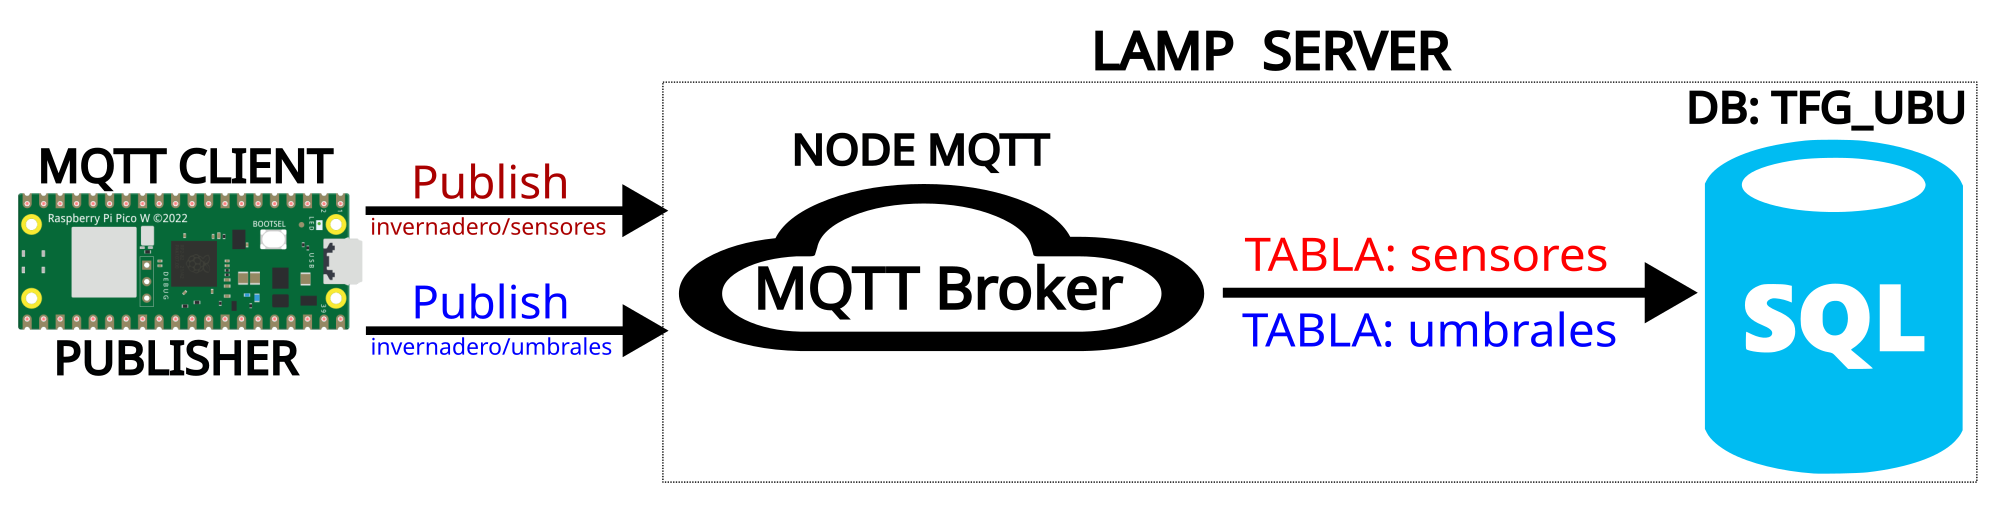
\includegraphics[width=1\textwidth]{img/diagramas/mqtt_nodeMqtt.png}
	\caption{MQTT con Node.js para almacenar datos de los sensores.}
\end{figure}

%Este apartado pretende recoger los aspectos más interesantes del desarrollo del proyecto, comentados por los autores del mismo.
%Debe incluir desde la exposición del ciclo de vida utilizado, hasta los detalles de mayor relevancia de las fases de análisis, diseño e implementación.
%Se busca que no sea una mera operación de copiar y pegar diagramas y extractos del código fuente, sino que realmente se justifiquen los caminos de solución que se han tomado, especialmente aquellos que no sean triviales.
%Puede ser el lugar más adecuado para documentar los aspectos más interesantes del diseño y de la implementación, con un mayor hincapié en aspectos tales como el tipo de arquitectura elegido, los índices de las tablas de la base de datos, normalización y desnormalización, distribución en ficheros3, reglas de negocio dentro de las bases de datos (EDVHV GH GDWRV DFWLYDV), aspectos de desarrollo relacionados con el WWW...
%Este apartado, debe convertirse en el resumen de la experiencia práctica del proyecto, y por sí mismo justifica que la memoria se convierta en un documento útil, fuente de referencia para los autores, los tutores y futuros alumnos.
